\documentclass[12pt,a4paper]{report}

% Packages
\usepackage[utf8]{inputenc}
\usepackage[T1]{fontenc}
\usepackage{graphicx}
\usepackage{amsmath}
\usepackage{amssymb}
\usepackage{caption}
\usepackage{subcaption}
\usepackage{hyperref}
\usepackage{fancyhdr}
\usepackage[top=2.5cm,bottom=2.5cm,left=3cm,right=3cm]{geometry}
\usepackage{titlesec}
\usepackage{lipsum}
\usepackage{float}

% Format
\pagestyle{fancy}
\fancyhf{}
\rhead{ELEC40006: EEESeaBoat}
\lhead{Group 14 Report}
\cfoot{\thepage}

% Title page
\title{\textbf{EEESeaBoat Project Report} \\ \large ELEC40006 -- Electronics Design Project 1}
\author{
\textbf{Group 14:} \\ David Lesman (CID: 02371181) \\ Thanus Palakumar (CID: 02556047) \\ Denzil Erza-Essien (CID: 02593040) \\ Lukas Mykhnenko (CID: 02579708) \\ \\ \\
\textbf{Word Count:} 9,228
}
\date{May/June 2025}

\begin{document}

\maketitle
\tableofcontents
\newpage

\chapter{Abstract}
This document details the design and construction of the EEESeaBoat, developed to scope out a simulated terrain filled with electronic ducks. Leveraging principles of circuit design, digital logic and programming, the objective was to design a robust and compact rover with relevant sensors. The primary aim was to be able to approach ducks, analyse them and provide feedback on their species and names.

Beyond detection, the project involved designing efficient code to control the rover's movement using an app, thus integrating concepts of low-latency wireless control, web interfaces and the integrated Wi-Fi module of a microcontroller. The fundamental design emphasizes cost efficiency and manoeuvrability within environmental constraints as real-world engineers would consider.

We abided by a structured process to ensure all design criteria and deadlines were met efficiently. The first phase was planning and research involved analysing components using theory and calculating appropriate values. The second phase was the design process which involved evaluating analogue against digital signal processing methods for detection systems and extracting the best ideas to ensure all criteria were met for the rover. Following this, we designed an interface for real-time user interaction and data analysis.

Finally, the hardware and software components were intertwined to execute the construction and movement of the final rover.

Testing demonstrated reliable detection of all 4 duck species as displayed on the interface with clear frequency measurements and name decoding within a total cost of roughly £45, highlighting the group's frugality.

\chapter{Introduction and Targeted Objectives}
The design process is streamlined into three technical components – Name Analysis, Species Analysis and Motion.

One major element of this task was therefore the designing and constructing of sensors for infrared waves, radio waves and magnetic waves respectively. With these, the EEESeaBoat would be able to classify the different ducks in the aquatic environment.

The ducks would also be communicating with “inaudible vocalisations” or ultrasonic signals which must be detected and decoded to identify their names. This key challenge of Name Analysis involves the understanding of resonant transducers, demodulating the amplitude-shift keying to extract the digital UART data and retrieving the names encoded as a 4-character ASCII string.

Naturally, a static rover with sensors and detectors is nothing short of a sitting duck. Hence, the final section concerns itself with motion. Using the EEBug design from the Autumn and Spring terms along with the Metro M0 microcontroller and Arduino code to implement a Wi-Fi based remote control system, the team also strived to design a user-friendly interface that not only provided a means of control but also information on the ducks. This underlying addition will help the team verify their success along the way.

The following information highlights the task objectives in further detail and the members responsible for executing it.

\section{Target Objectives}

\subsection*{Infrared Detection (Thanus)}

The ducks will be emitting infrared pulses, which we will need to detect using a phototransistor. Beyond infrared detection, this task involves balancing technical requirements with practical constraints, necessitating an optimized detection strategy within the given time constraints.

Four distinct duck species are characterized by specific frequencies with the Wibbo and Snorkle serving as the detection targets. This accentuated the need for a filter, to ensure the sensor would only be sensitive to the wavelength of the duck`s emission. Another stipulation is that the habitats emit light of a different frequency while the ducks emit optical power weaker than standard light sources, reinforcing how our detection must be accurate and make measurements within appropriate bounds.

Due to the potential for frequency deviations and simultaneously needing to avoid unwanted frequencies, the detection system must accommodate a narrow acceptable range of results. To ensure clear signal analysis, the design will adhere to a detect-amplify-filter setup.

\subsection*{Ultrasonic Detection (Denzil)}

The ultrasonic detection task requires detection of a high frequency analogue signal which must be converted to a digital signal. Using this digital signal, the binary output can be used to convert this into letters, entailing the names of the ducks.

This task required further research on ultrasonic signals and detection making it the largest challenge and most time-consuming sub-task of this overall section. However, the rest of this challenge used simpler concepts built upon prior to the project such as amplification, envelope detection and frequency filtering.

The output of this is then fed into the RX port of the Arduino, which has a built-in function to decode the UART signal.

\subsection*{Magnetism Analysis (Lukas)}

The magnetic detection task presents unique challenges due to the static nature of the duck's magnetic field. Unlike dynamic fields that induce currents in coils, our solution must detect a fixed magnetic orientation without movement. This means practical implementation favours Hall effect sensors. The key challenge lies in reliably detecting weak magnetic fields at varying distances while accurately determining polarity.

Our approach must balance several competing factors: sensitivity to detect the field at practical distances, precision to determine orientation accurately, and immunity to environmental interference. The solution will have to involve a combination of sensor selection, careful positioning, and signal conditioning. The high-sensitivity DRV5053 hall effect sensor offers a promising starting point, but it requires additional amplification to achieve detection at reasonable distances.

Testing will be critical to validate detection range and orientation accuracy under realistic conditions. The final implementation must accommodate potential field strength variations while maintaining consistent polarity detection - a task that may require adjustable thresholds in our microcontroller code.

\subsection*{Arduino and CAD (David)}

Once all signals have been received, the Arduino is responsible for translating them to meaningful data. Each tool has its own function in code that decodes the signal, and meaning, which sends it through to a user interface. The Arduino is also responsible for receiving user commands from the interface and translating that to appropriate commands to read from each tool or move the motors a certain way.

As this is a big project, we felt to simplify the process we would use the existing chassis, with some added mounts to place the appropriate detectors and extra space for more circuitry in the form of a shelf to place a breadboard.

\subsection*{Radio Detection (Denzil + David + Thanus)}

The species of ducks rely upon multiple detection mechanisms and the second of them is radio wave sensors. To detect the remaining 2 species, the detection system must receive and decode amplitude-modulated signals transmitted by the ducks. With careful selection of components, the key objective is to extract our desired information and frequencies from the duck signals by converting radio waves into usable signals.

This procedure will involve an RLC filter to ensure resonance occurs at the target 89kHz frequency and the circuit is not interrupted by undesired frequencies before being followed up by the diode responsible for demodulation. Like the IR section, the final signals will be weak for detection, hence relying upon op-amps to strengthen the signal before feeding it into the Metro M0 microcontroller for digital analysis. Certain aspects mimic the IR section, however this detection system requires greater attention to filters and demodulation compared to a simple phototransistor-amplification-filter system. Another note would be positioning on the rover: both IR and radio systems will be measuring incoming waves from the ducks however radio waves have a greater wavelength hence it is more convenient to position the radio detection system behind the IR system to ensure directional equity rather than equality.

\subsection*{Report (Thanus + David)}

Throughout the project, logs will be made of planning, progress and challenges to overcome which will simultaneously be documented as a 10,000-word report. This document intends to clearly convey both theory and practical elements of the group project. Following a clear structure of highlighting objectives, analysing theory and plans, practical evaluation and closing judgments, the aim is to set out the research in a professional and sophisticated matter for an expert audience.
\chapter{Project Management and Team Coordination}
Before starting the project, as a group ,we deemed it integral to discuss and formulate an effective plan which played to everyone’s strengths as well as allowing for reasonable time to complete sub-tasks. A Gantt chart (shown below) was formed to help assign tasks, allowing for clear roles to be set as well as their time constraints:

\begin{figure}[h]
    \centering
    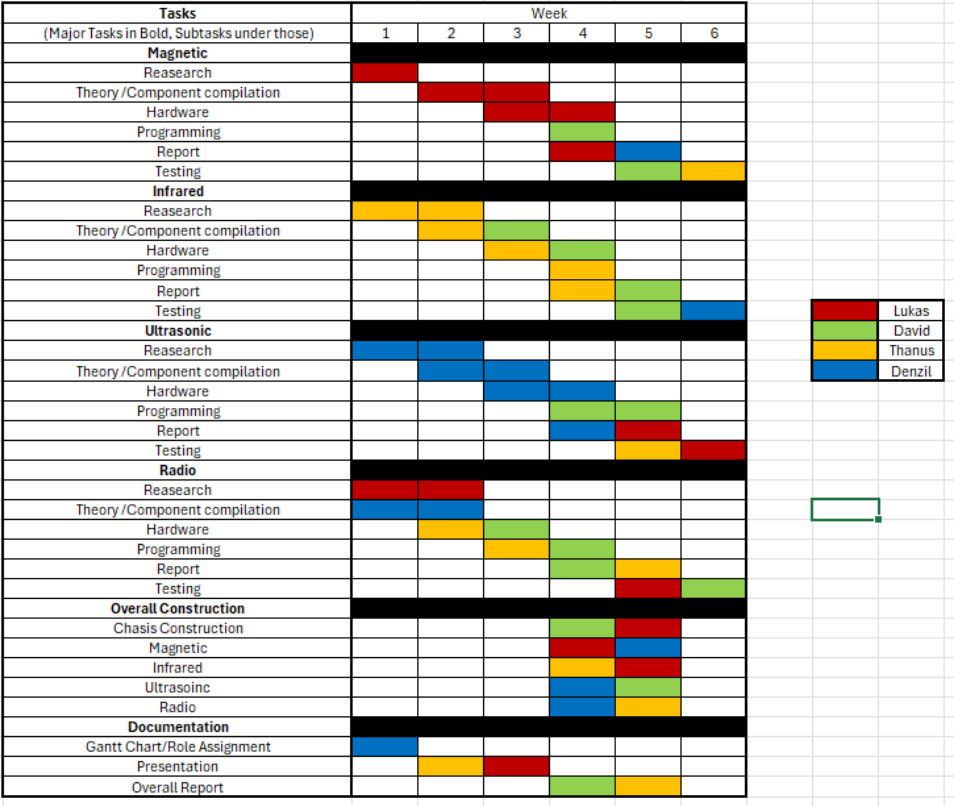
\includegraphics[width=0.8\textwidth]{subpages/images/gantt_chart.png}
    \caption{Gantt Chart}
    \label{fig:gantt}
\end{figure}

Key things to note from this Gantt chart and the subsequent planning include:
\begin{itemize}
    \item The `Overall Construction' main task and `Testing' subtasks were purposely handled by two people each in which those selected hadn’t done the other task for that specific part of the project (i.e. two people constructing the magnet circuit wouldn’t be responsible for testing the circuit). This was done to remove any potential bias, whether deliberate or otherwise.
    \item This chart was the final edition as if tasks, when practically worked on, were deemed as trivial, this would give members in the group spare time allowing for further collaboration in the more time-consuming subtasks of the project.
    \item Most importantly, this plan does not restrict members of the team moving and assisting other members with their construction or testing. Though, this should only be if they have made sufficient progress or completed their own section.
\end{itemize}

% Placeholder for next chapters
\chapter{Infrared Detection}
\section{Initial Ideas}
This task concerns itself with detecting two specific infrared frequencies to differentiate between the species of Wibbo and Snorkle. The first idea was just to test the phototransistor with no modifications whatsoever to gauge a sense of the accuracy. When the transistor was placed against the duck’s neck, our program detected frequencies which were outputted on our terminal, but they were sporadic and fluctuating between extreme values. Furthermore, at even a little distance away, signals could not be detected at all. The initial stance was therefore clear, we needed to amplify the signals from the phototransistor, and we needed to filter frequencies to get stable, accurate readings.

\section{Dissecting the Phototransistor}
\begin{figure}[h]
    \centering
    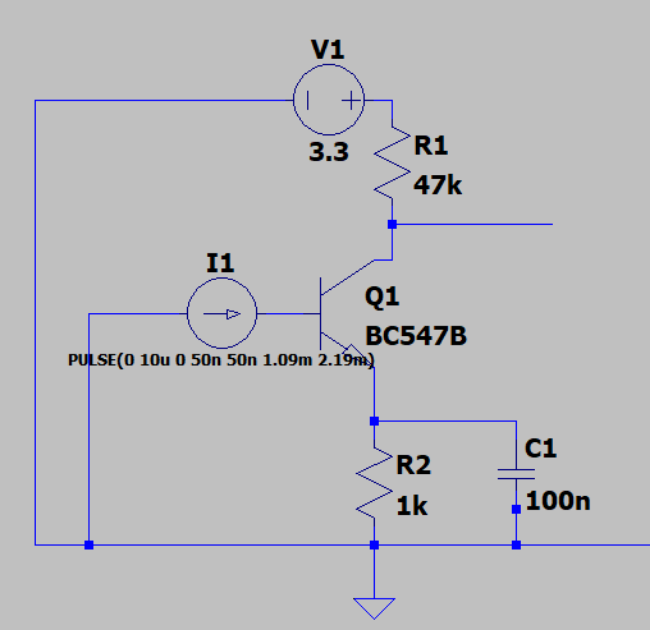
\includegraphics[width=0.8\textwidth]{subpages/images/phototransistor.png}
    \caption{The Phototransistor}
    \label{fig:phototransistor}
\end{figure}

The phototransistor is an electrical device that uses incoming light on its base and converts photons into electrons. By the photoelectric effect, light photons with adequate energy to exceed the work function excite electrons. This base current is amplified to produce a larger collector current. The design above mimics that of a common-emitter amplifier, where the wire drawn from the collector is to be amplified in the forthcoming stage.

The structure evident in Figure 2 involves an emitter degeneration resistor - as the emitter current rises, the voltage across Re rises and this in turn lowers the base-emitter voltage. This biases the transistor to prevent fluctuations in collector current and maintains thermal stability of the circuit. Biasing the input at Vbe is unwise given that several parameters vary with temperature. The negative feedback of the phototransistor ensures that the current generated stays within bounds.

The electrolytic capacitor boosts the gain by maintaining the biasing and attenuating AC signals. This introduces the low-pass filter for high-frequency noise early on to limit the frequencies we will be analysing.

A key adaptation is the pulse signal applied to the base. LTspice does not allow for simulation of light, but we are told that the duck emits pulses of infrared light. In Figure 3, the current source uses rise time and fall time of 50 nanoseconds with a full time-scope of 10 microseconds. Most importantly is the 2.19 millisecond period derived from the frequency of the 457Hz as period is the reciprocal of frequency - the pulse in LTspice mirrors the likely pulse emitted by the Wibbo.

\begin{figure}[h]
    \centering
    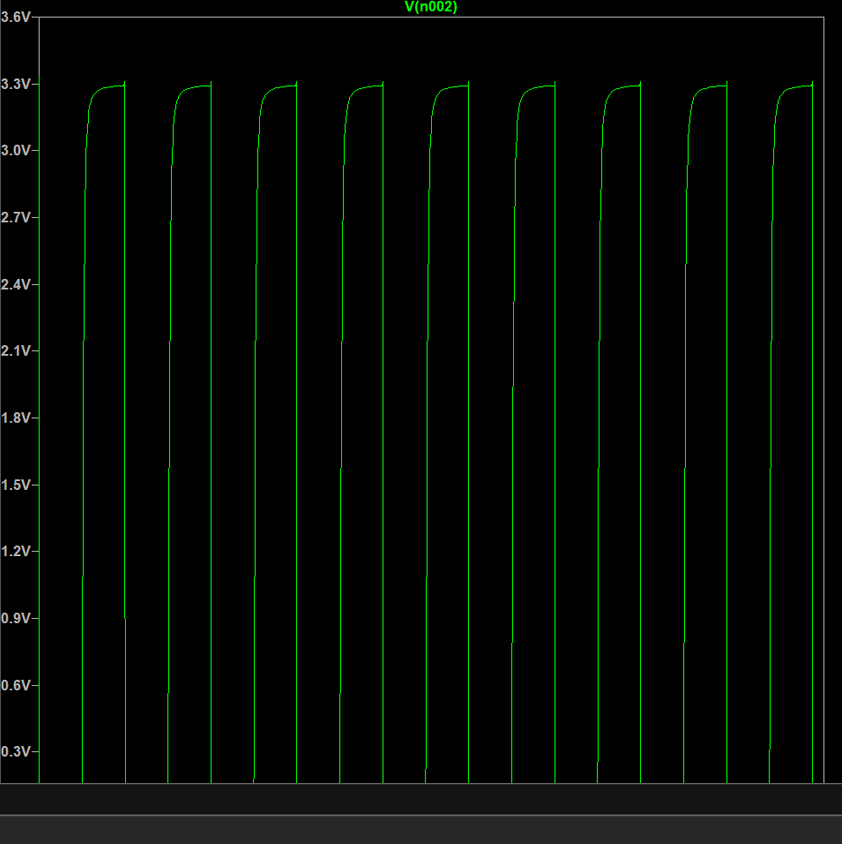
\includegraphics[width=0.8\textwidth]{subpages/images/pt_transient.png}
    \caption{Transient Analysis of Phototransistor}
    \label{fig:phototransistor_transient}
\end{figure}

Any transistor would be expected to amplify the signals it receives by set degree. Whilst the transient simulation above shows that the output voltage signal is square-like and around 3.3v amplitude which is what we desire – there are a couple of issues that deem this circuit inadmissible.

Issue 1: We are assuming that all the light directly hits the base when the light might scatter or potentially reflect meaning that our actual voltage output signal is far weaker.

Issue 2: Looking carefully at the peaks and troughs, we see that they do not perfectly mirror a square wave - there is overshooting and undershooting due to parasitic capacitance – a transistor in its switching process causes the voltage to stray from its bounds.

Issue 3: Though the waveform seems fine, there is an inverse relationship causing problems. When light hits the transistor, conduction causes the collector current to flow through the transistor to the ground. The voltage at the collector drops because the system sinks current. However, we would ideally prefer light hitting to cause a high voltage, so an inversion technique is required.

To ensure signals can be easily detected and follow correct logic, we must therefore consider the next phase of this design - the amplification stage.

\section{Amplification Analysis}
Following the phototransistor stage, the signal needs to be amplified given that it is currently too small for detection and may lead to our duck signals going under the radar. However, we also need to invert the waveform since the phototransistor operates under the basis of high light intensity leading to a low collector voltage. A non-inverting amplifier would result in a low pulse for the frequency detected and a high pulse for the light not detected. Whilst this remains easy to interpret, it is still inconvenient hence the need for our group to use an inverting amplifier as in Figure 4.4.

\begin{figure}[h]
    \centering
    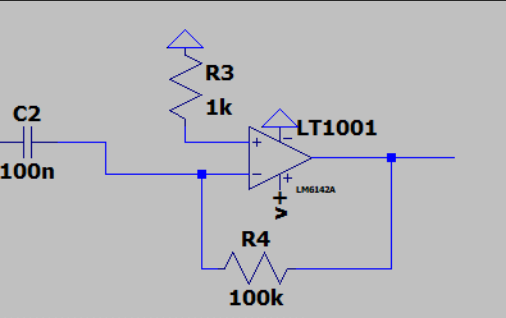
\includegraphics[width=0.8\textwidth]{subpages/images/amplification_stage.png}
    \caption{Transient Amplification Stage}
    \label{fig:amp_stage}
\end{figure}

Another component that has been added is the capacitor. This acts as a filter to attenuate ambient light changes but more importantly, remove DC bias. Selecting too high of a capacitance would increase the time constant and longer discharging would cause lag to the pulses.

To ensure clear detection, we have used a feedback resistor of 100k and a Rin of 1k to give a gain of -100. This helps us achieve the correct waveform pattern and ensures the voltages are sufficient for detection, especially when the ducks stray further from the infrared detector system.

\section{Complexities using Band-Pass Filters}
With the amplification side completed, we now needed to closely inspect the frequencies we are after. For this, there were several filters to consider but through this sub-section, we will reach an interesting conclusion.

First, we considered the passive filters and targeted a bandpass filter, depicted in Figure 5, as a standard low-pass filter or high-pass filter would not be sufficient. The bandpass is not between the Snorkle and Wibbo frequencies but rather the limits are set by our acceptable range for each frequency should it deviate. A Wibbo has 457Hz, so we set a 10Hz allowance either side and set the cutoff frequencies as 447 and 467 during the simulations demonstrated in Figure 4.6.

\begin{figure}[h]
    \centering
    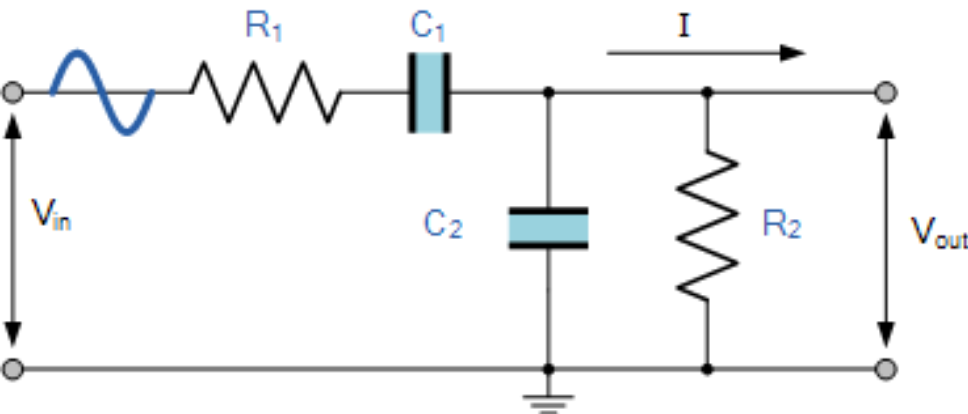
\includegraphics[width=0.8\textwidth]{subpages/images/passive_bp_filter.png}
    \caption{Passive Band-Pass Filter}
    \label{fig:passive_bp_filter}
\end{figure}
\begin{figure}[h]
    \centering
    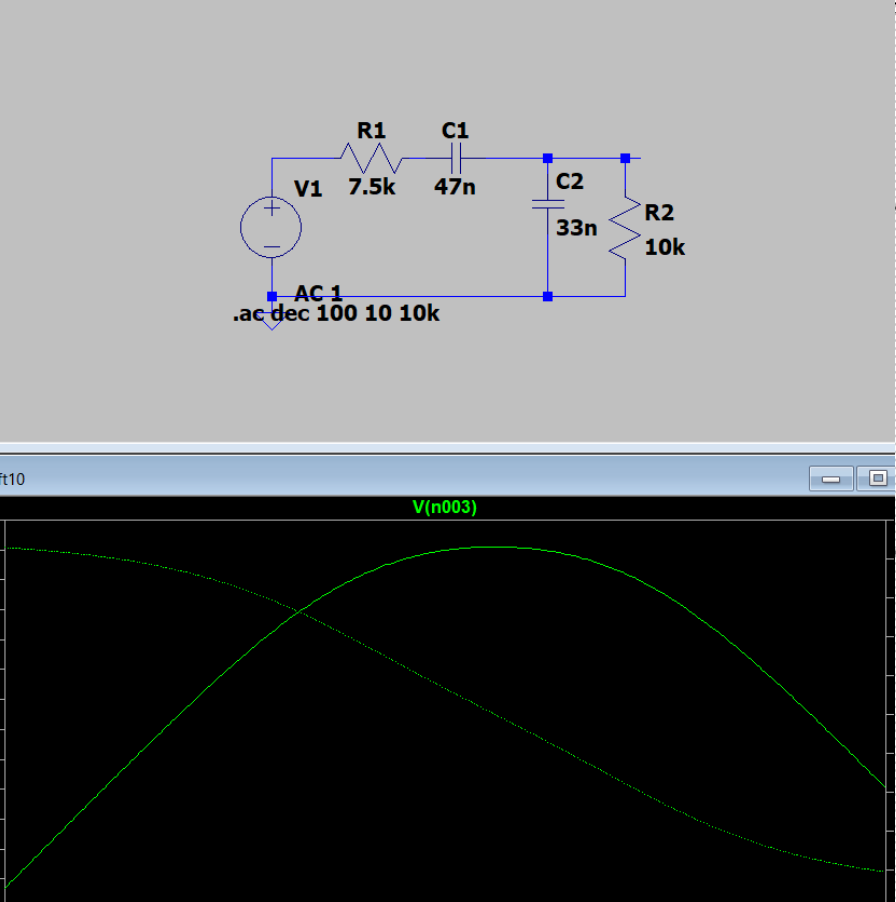
\includegraphics[width=0.8\textwidth]{subpages/images/test_passive_bp.png}
    \caption{Testing Passive Band-Pass Filter}
    \label{fig:passive_bp_filter}
\end{figure}

The calculations are as followed for the high-pass and low-pass filters.
\begin{enumerate}
    \item High-Pass Filter
          The cut-off frequency is given by \(f_c = \frac{1}{2\pi RC}\).
          For our values, R = 7.5k$\Omega$ and C = 47nF, this gives a cut-off at approximately 451.2Hz, which is within 0.94\% of the target 447Hz.
    \item Low-Pass Filter
          We have values R = 10k$\Omega$ and C = 33nF. This gives a cut-off at approximately 482.8Hz. This is is within 3.39\% of the target 467Hz.
\end{enumerate}

However, whilst passive filters are simpler and require less power, they cannot provide gain and rely on large inductor and capacitor values to function effectively. These components dissipate more energy near resonance, and such losses reduce the system's ability to sustain resonance.
\begin{itemize}
    \item A low Q means the circuit does not respond strongly to its natural frequency.
    \item Therefore, the filter allows a broad range of frequencies near the cutoff
    \item This results in a non-sharp cutoff; the transition from passband to stopband is gradual, not steep.
    \item Without amplification, any small energy losses cannot be corrected, meaning the filter is not sharply selective.
\end{itemize}

\begin{figure}[h]
    \centering
    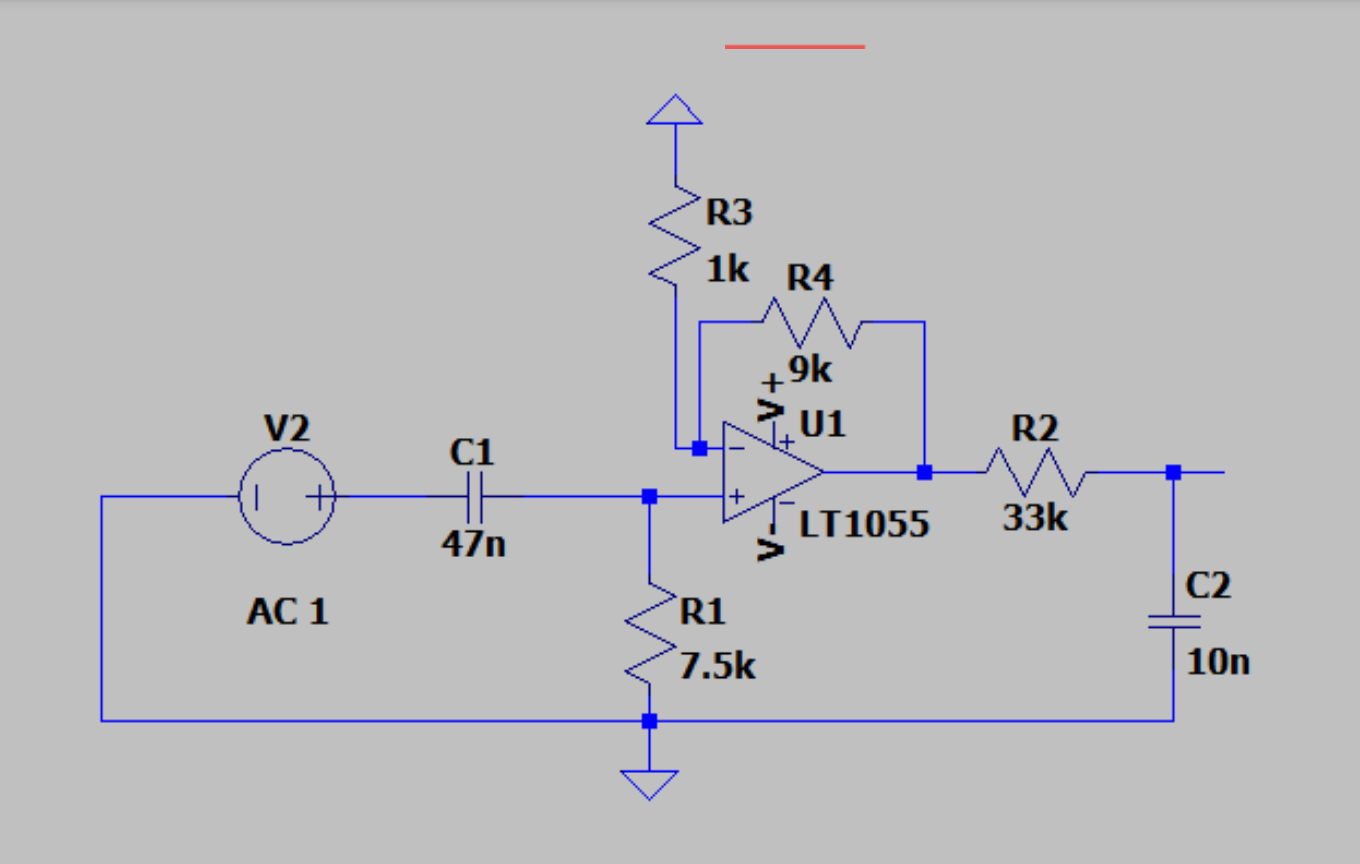
\includegraphics[width=0.8\textwidth]{subpages/images/non-invert-active-bp-filter.png}
    \caption{Non-Inverting Active Band-Pass Filter}
    \label{fig:active_bp_filter}
\end{figure}
\begin{figure}[h]
    \centering
    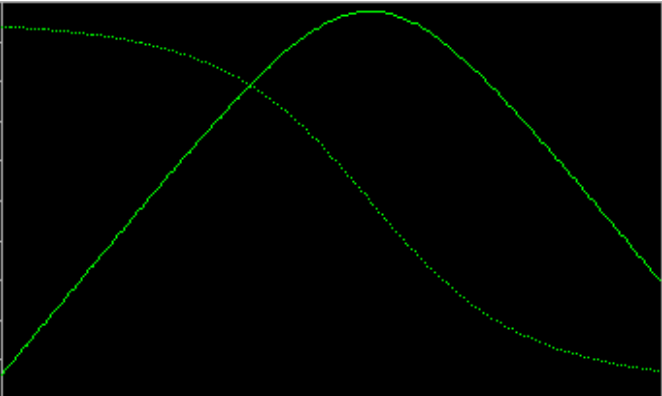
\includegraphics[width=0.8\textwidth]{subpages/images/ir_result_1.png}
    \caption{Simulation Results}
    \label{fig:simul_result}
\end{figure}

The circuit in Figure 4.6 represents a non-inverting active band-pass filter re-using the components calculated from earlier but now including an op-amp. We have the high-pass filter first, then the amplification and finally the low-pass filter. R3 and R4 also work together to give us a gain of 10 - calculated by \(1+ \frac{R_f}{R_{In}} \) - which is reasonable and can always be adjusted if there is clipping.

Though we would expect a flat band-pass, we have also picked quite a narrow range for the cutoff frequencies - hence why the AC sweep in Figure 10 shows the right peak at 20dB but a swift rise and fall.

The last strategy was the Sallen-Key band-pass filter. The second-order filter can be precisely tuned using resistor and capacitors, leading to a potential symmetrical bell-shaped response for AC sweep. It also involves positive and negative feedback to shape the frequency. However, as clear below in figure 4.8, the circuitry becomes quite overwhelming.

\begin{figure}[h]
    \centering
    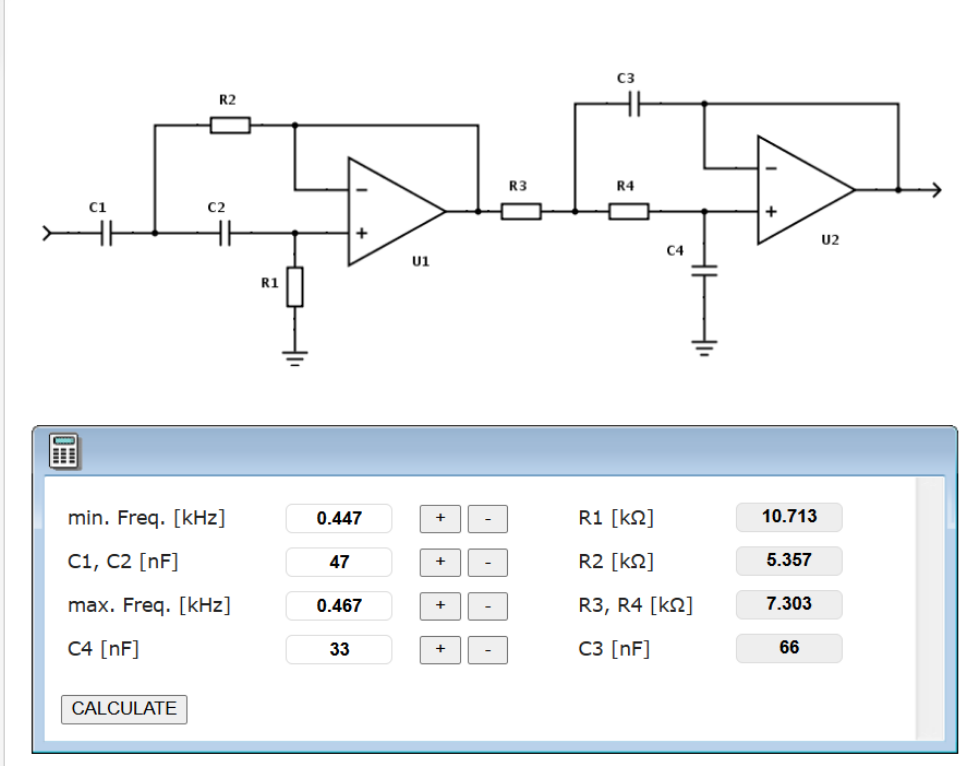
\includegraphics[width=0.8\textwidth]{subpages/images/sallen_key.png}
    \caption{Sallen-Key Analysis 1}
    \label{fig:sallen_key}
\end{figure}

The following simulation on LTspice show the peak frequency at around 458Hz and our target for the Wibbo was 457Hz implying that the Sallen-Key is filtering correctly and provides a nice bell-shaped symmetrical frequency response.

\begin{figure}[h]
    \centering
    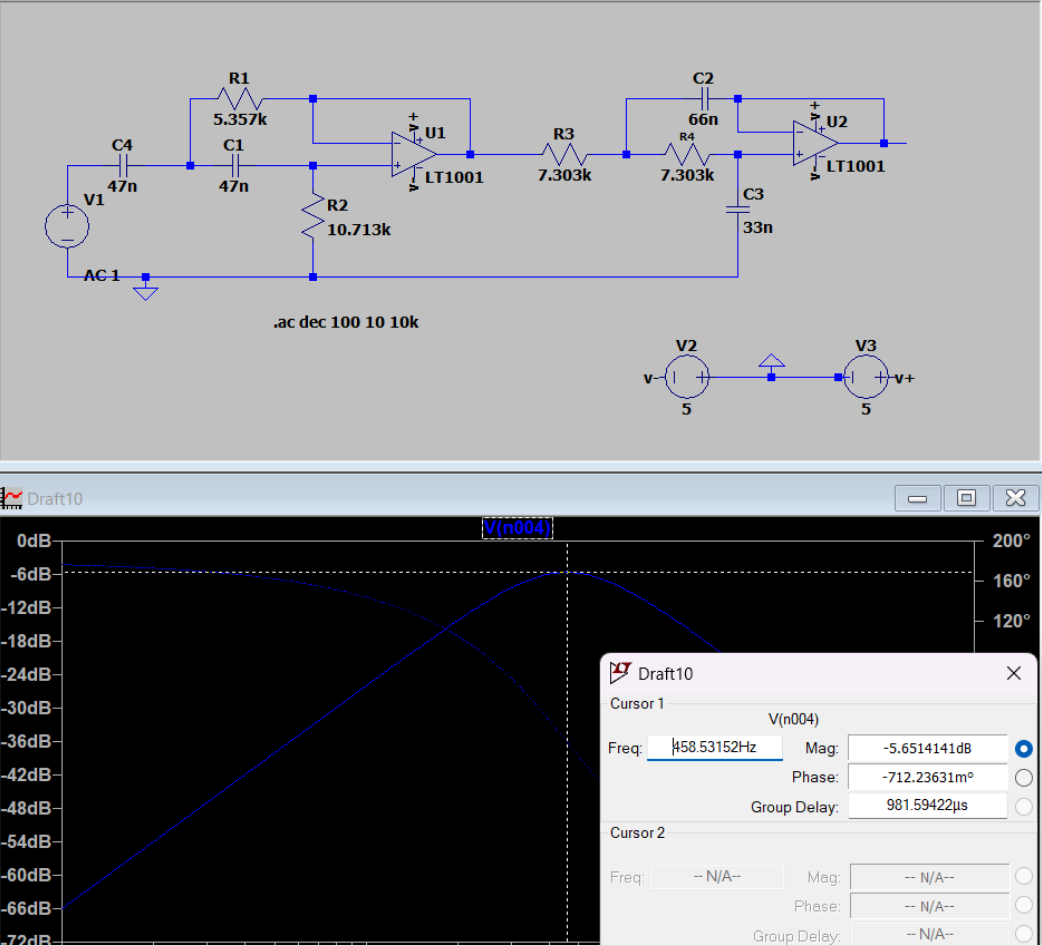
\includegraphics[width=0.8\textwidth]{subpages/images/sallen_key2.png}
    \caption{Sallen-Key Analysis 2}
    \label{fig:sallen_key2}
\end{figure}

Despite this, the issue should be clear by now. We need to utilise two band-pass filters to account for both Wibbo detection and Snorkle detection, which will make this circuit severely complicated. When using LTspice, the final hypothetical circuit would look like the diagram on the next page.

Following this, the conclusion was that hardware was going to take up space and get complicated very quickly. To mitigate the complexities, we needed to think of a method that took less time, not as complicated and helped us get the frequencies we needed. The solution to this was turning to our Arduino code.
\begin{figure}[H]
    \centering
    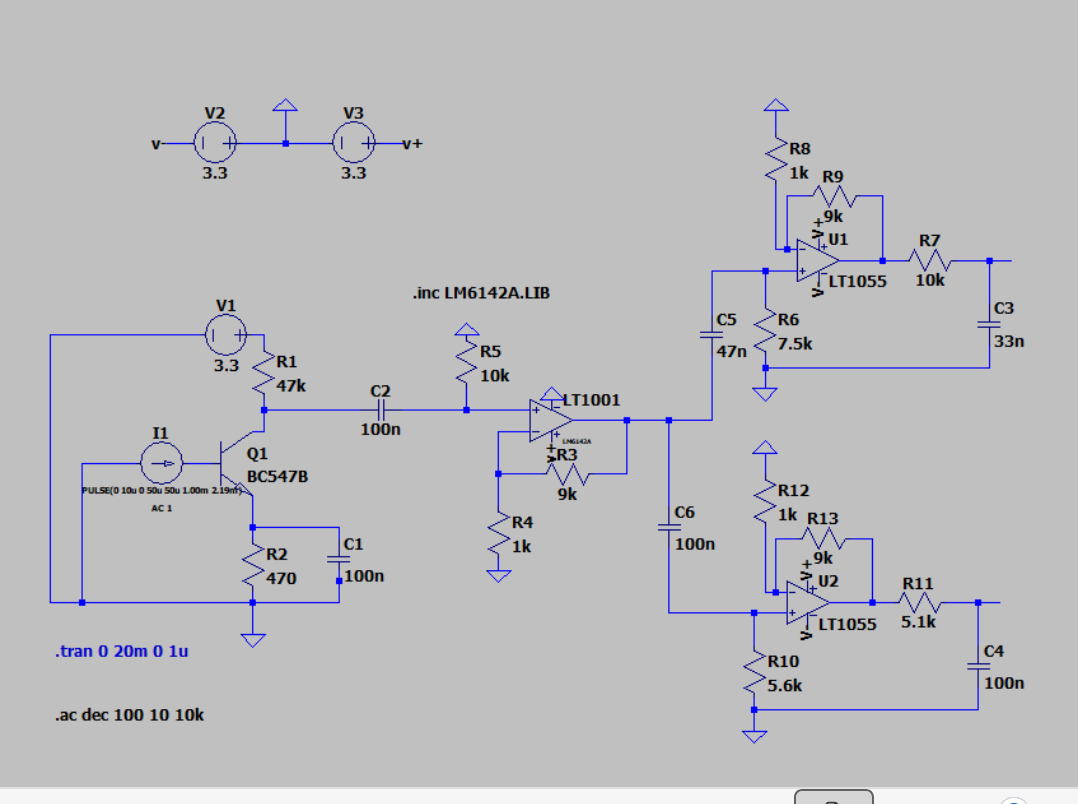
\includegraphics[width=0.8\textwidth]{subpages/images/ir_complex.png}
    \caption{Complete Circuit Diagram - For Analysis Only}
    \label{fig:complex_circuit}
\end{figure}

Before that, another sidenote would be the selection of the LM324N operational amplifier. Whilst alternatives like ADA4817 and OPA3333 were evaluated for their higher bandwidth, lower noise, and favourable slew rate, they were both surface mounted. This means they sit on a PCB and do not have flexible leads which, on top of being exceedingly small, make them difficult to work and test with plus if damaged could harm our budgeting.

The LM324N offers an output swing between -1.5v to 1.5v with a 5v single supply which preserves signals, without clipping, even at extremely low supply voltages. Furthermore, the infrared pulses that hit the phototransistor will produce weak transient signals that require amplification without distorting harmonies. The gain-bandwidth product for this op-amp is 1MHz meaning that for the short pulses, which contain a multitude of frequency components beyond the fundamental, this modest GBP can ensure the op-amp maintains signal integrity and effectively manages the signal bandwidth during said amplification.

Noise performance also represents a critical consideration in the characteristics of this op-amp. The LM324N exhibits an input bias current of 45nA with temperature compensation, and an input offset voltage of just 2mV. While these specifications may not complete match the requirements of precision amplifiers, they prove sufficient given the signal levels being dealt with.

The selected op-amp also demonstrates excellent phase margin characteristics, maintaining stability even when driving capacitive loads at the output stage. This robustness against oscillation ensures clean, undistorted signal regeneration without the need for further, complicated stabilization networks.

Thus, though trade-offs were required, the LM324N presented itself most favourable for this detection system and depicted below for practical reference.

\begin{figure}[H]
    \centering
    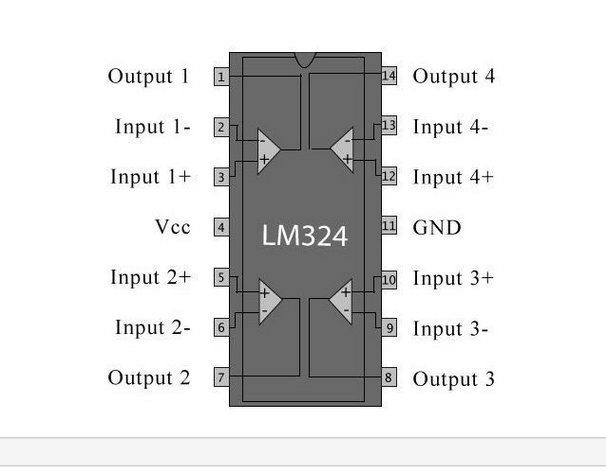
\includegraphics[width=0.8\textwidth]{subpages/images/lm324n.png}
    \caption{LM324N Cross-Section}
    \label{fig:lm324n}
\end{figure}

\section{Simplification using Arduino}
After discussing with a member of staff, Dr Hakan Merdan, the team unanimously agreed that there was a way to manipulate the Arduino code to our advantage. Though the full, updated code will be discussed later, the following snapshot depicts an earlier version of this key section.
\begin{verbatim}
// Check for Wibbo: 447-467Hz
if (frequency >= 447 && frequency <= 470) {
    response += "It's a Wibbo!";
}
// Check for Snorkle: up to 303Hz
else if (frequency >= 283 && frequency <= 303) {
    response += "It's a Snorkle!";
}
\end{verbatim}
Our original method of analogue filtering involved two band-pass filters which would avoid software processing delays and identify species well, but the circuitry is complex, has limited flexibility and components can be very sensitive.

Our upgraded method of digital signal processing uses \texttt{pulseIn()} to measure high/low amplified phototransistor signals. The following line:
\begin{verbatim}
float frequency = 1000000.0 / (highTime + lowTime)
\end{verbatim}
calculates the frequency of the pulses mathematically while the snapshot above compares against the expected range. Note that we have not targeted the specific species-related frequency but instead allowed for a range due to deviations in the signal frequency.

This tactic involves simpler hardware, reduced space and weight, flexible thresholds using small change in code and no risk of errors due to parasitic impedance or capacitance of components. However, software implementation does possess limitations such as timing inaccuracies when handling multiple asynchronous sensor inputs. With several sensors sending data that the Arduino needs to read and interpret, the interface may experience a slight lag.

Our final circuit -- with no filters and output to be connected to our Metro M0 microcontroller -- therefore looks like this with the supporting transient simulation:
\begin{figure}[h]
    \centering
    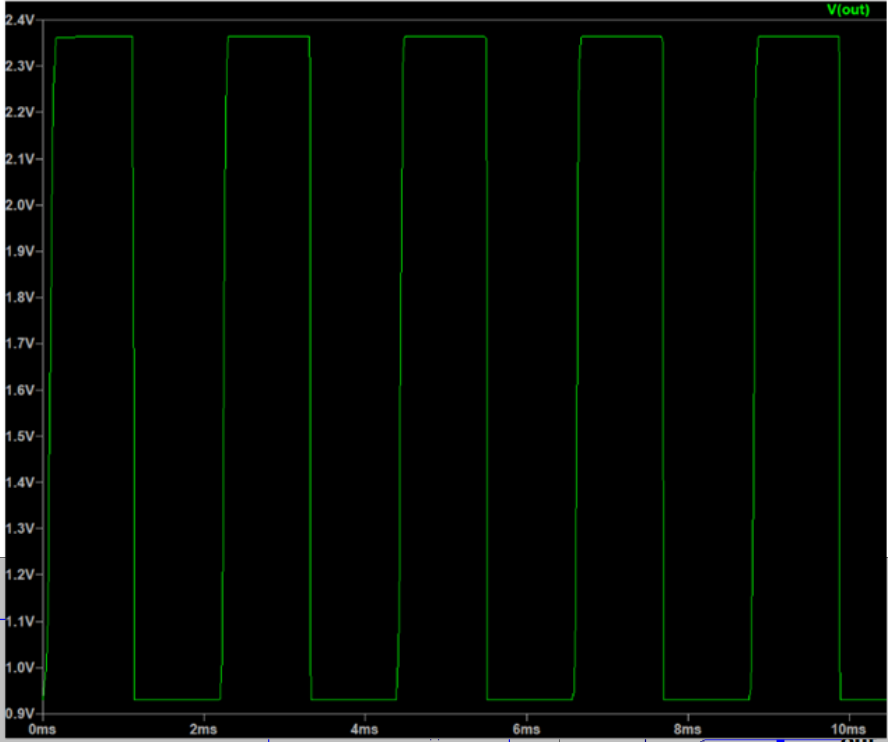
\includegraphics[width=0.8\textwidth]{subpages/images/ir_expected.png}
    \caption{Expected Results from Simulation}
    \label{fig:expected_results}
\end{figure}
\begin{figure}[h]
    \centering
    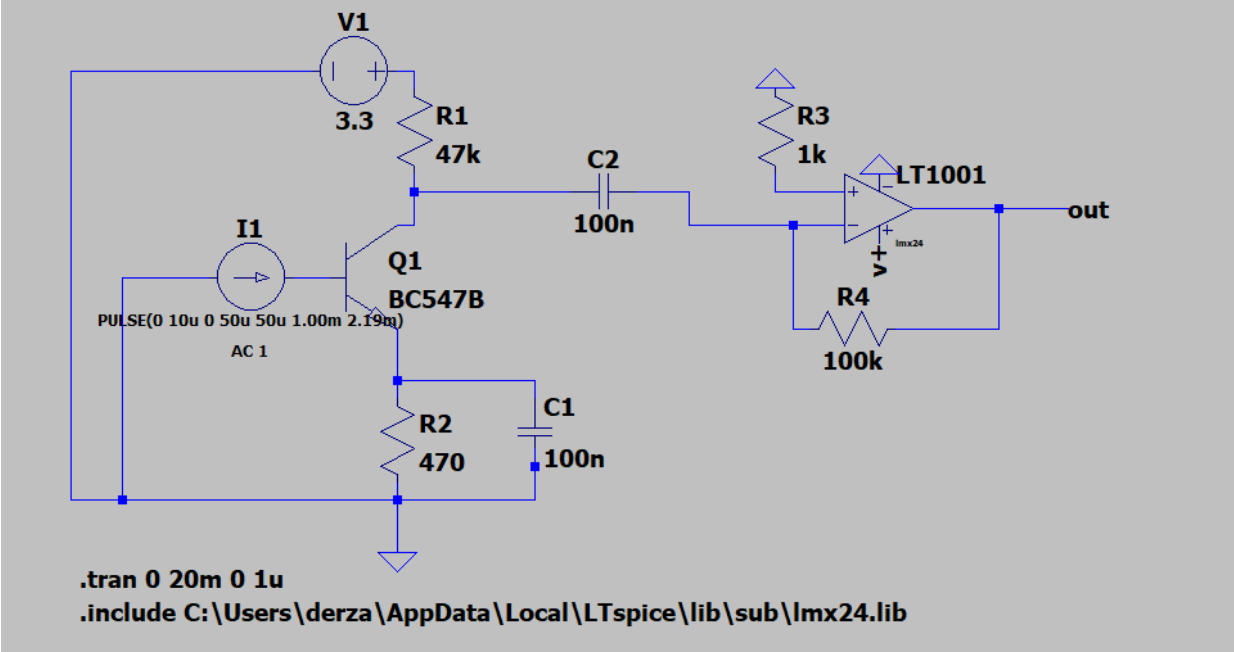
\includegraphics[width=0.8\textwidth]{subpages/images/ir_final.png}
    \caption{Final SPICE Circuit for IR Detection}
    \label{fig:final_circuit}
\end{figure}

The procedure flowchart below clearly summarizes the steps that have and will be taken in this Infrared Detection task.
\begin{figure}[h]
    \centering
    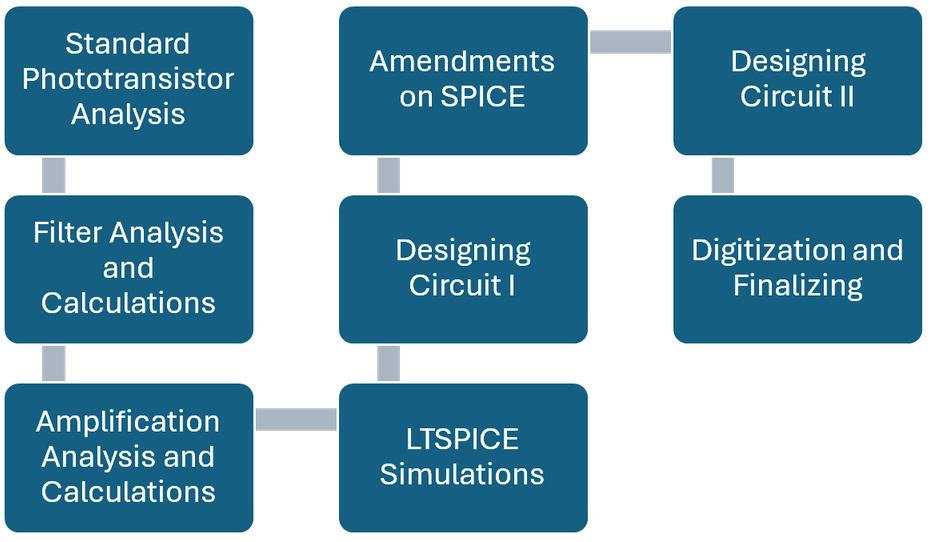
\includegraphics[width=0.8\textwidth]{subpages/images/ir_procedure.png}
    \caption{Infrared Detection Task Flowchart}
    \label{fig:ir_flowchart}
\end{figure}
\begin{figure}[h]
    \centering
    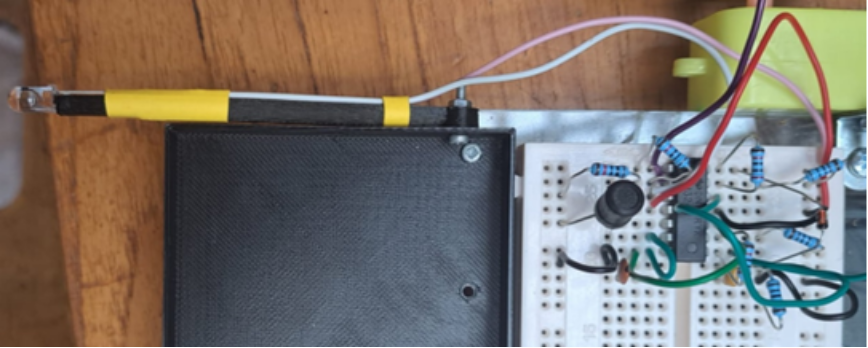
\includegraphics[width=0.8\textwidth]{subpages/images/ir_irl.png}
    \caption{IR Circuit}
    \label{fig:ir_circuit}
\end{figure}

\section{Building and Testing}
The breadboard circuit constructed led to successful practical simulation where the sharp pulses were detected on this oscilloscope. Evidently, these pulses starkly contrast the square pulses we expected from the SPICE simulation. In real hardware, the IR light from the ducks is emitted in sharp bursts compared to perfectly square waveforms. Building on this, the phototransistor response is rapid and therefore the oscilloscope showed the narrowest part of the signal. Other reasons could have been the bandwidth limits compressing the rising and falling edges into narrower spikes.
\begin{figure}[h]
    \centering
    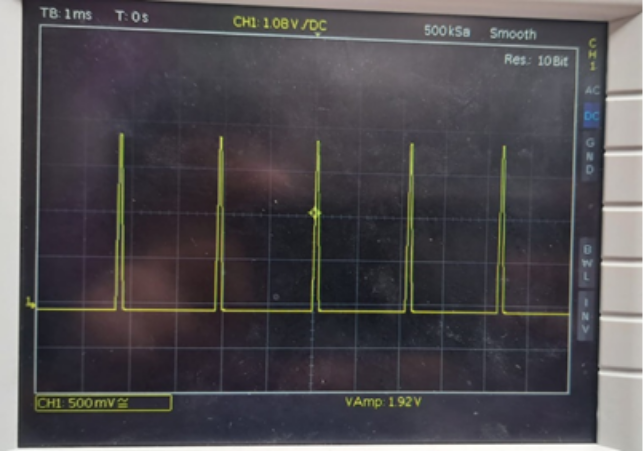
\includegraphics[width=0.8\textwidth]{subpages/images/ir_probe.png}
    \caption{Results for Probing IR Circuit}
    \label{fig:ir_probe}
\end{figure}

Regardless, the pulses in Figure 4.16 are still exhibited when the phototransistor is within reasonable proximity of the ducks leading to our interface correctly outputting the species and respective frequency.

However, initial analysis revealed that there was a minor inconvenience to our detector. Whilst the IR light was detected at a sufficient distance, the pulses were far weaker at first. This result contradicted the idea of amplification and led to circuit checks which were to no avail. Eventually, it became apparent that when there was a cover over the transistor, the pulses are as seen in the image but weaker and less clear when completely exposed. The ambient light from the room was most likely interfering because whilst we have digitally filtered the frequencies, the oscilloscope-probing process is independent of that. Hence, this led into the next step – design a cover to ensure other frequencies are not interfering with our IR detector.

With the desired signal, the detection system is complete for the Wibbo and Snorkle species. This was an example of species detection which will be returned to, but the next section concerns itself with name identification.


\chapter{Ultrasound Detection}
\section{Initial Ideas}
The duck's name is encoded as ASCII characters and framed as UART packets in an ultrasonic signal.
\begin{figure}[h]
    \centering
    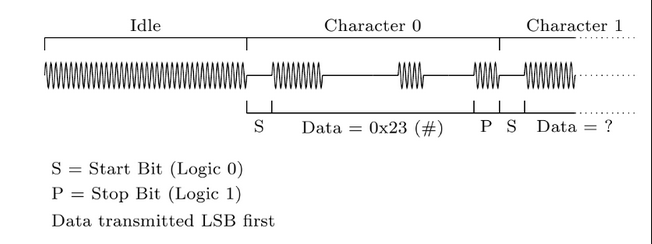
\includegraphics[width=0.8\textwidth]{subpages/images/ultra_spec.png}
    \caption{Model for the Output of the Duck's Name [2]}
    \label{fig:ultrasound_specifications}
\end{figure}

The communication works as such:
\begin{itemize}
    \item The start bit, S, indicates the start of an ASCII character
    \item The next bits will then produce a character, to indicate the letter. This can be seen in character 0 where the data is equal to 0x23, this is hexadecimal for the ASCII character `\#'.
    \item The last bit, P, is the stop bit indicating the end of an ASCII character (Note that each duck's name will start with the `\#').
\end{itemize}

To obtain these bits, an ultrasound transducer is used to pick up the ultrasound signal of the duck. This signal is then demodulated and converted to a binary signal using a comparator. The output from the comparator is connected to the microcontroller which has UART communication built in decoding the binary signal into bytes.

The overall circuit shown below can be split into 3 stages: the ultrasound signal (and amplification); the envelope detector; and the comparator circuit via a Schmitt trigger. These combine to give the desired bitwise logic shown in figure 5.2.
\begin{figure}[h]
    \centering
    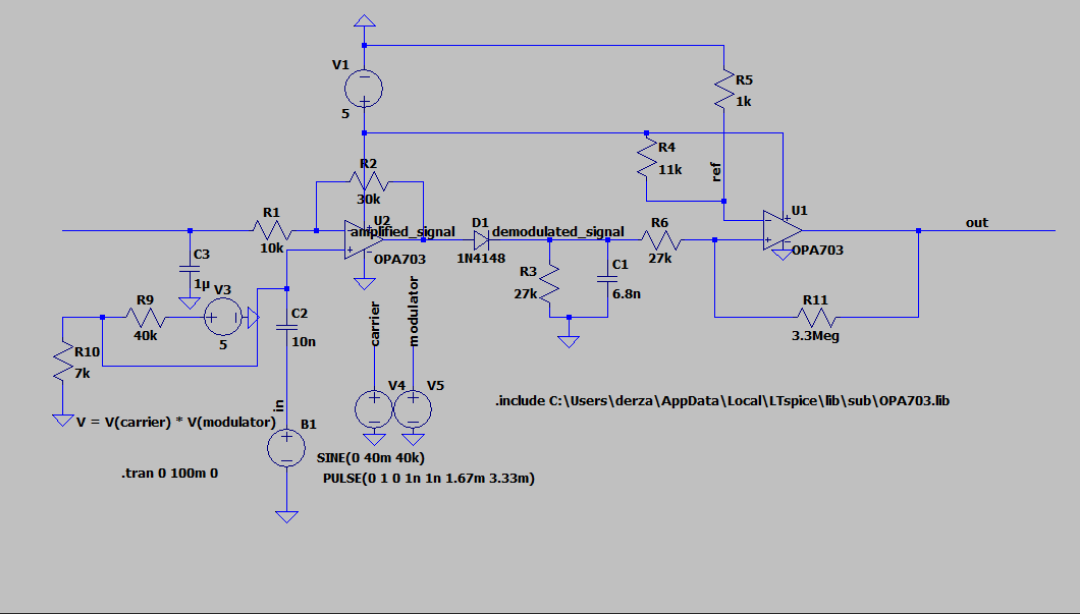
\includegraphics[width=0.8\textwidth]{subpages/images/ultra_circuit_naming.png}
    \caption{LTspice Circuit Diagram for the Duck Naming Process}
    \label{fig:ultrasound_naming_circuit}
\end{figure}

\section{The Ultrasound Signal}
The ducks communicate using a carrier frequency of 40kHz modulated with a form of amplitude-shift-keying (ASK), where an amplitude of 0 represents logic 0 and an amplitude much greater than 0 represents logic 1.

A piezoelectric transducer was used as it operates around the required level and can effectively convert mechanical vibrations into electrical signals [3]. Moreover, as they have a high range of frequencies, i.e. they can measure a large range, they are the most ideal transducers.

The MCUSD16A40S12RO [4] transducer was selected due to its high sensitivity as well as being compact and lightweight. Moreover, it has a low power consumption, which is a benefactor for our high efficiency target.
\begin{figure}[h]
    \centering
    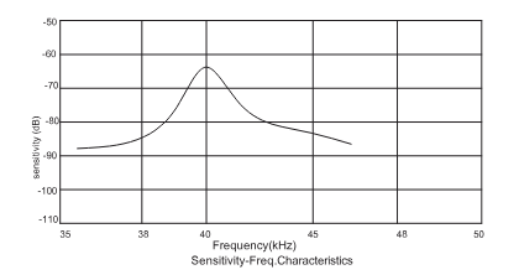
\includegraphics[width=0.8\textwidth]{subpages/images/ultra_sensitive_freq.png}
    \caption{Sensitivity-Frequency Graph for MCUSD16A40S12RO}
    \label{fig:sensitivity_frequency}
\end{figure}

This transducer was tested practically, giving the signal shown below.
\begin{figure}[h]
    \centering
    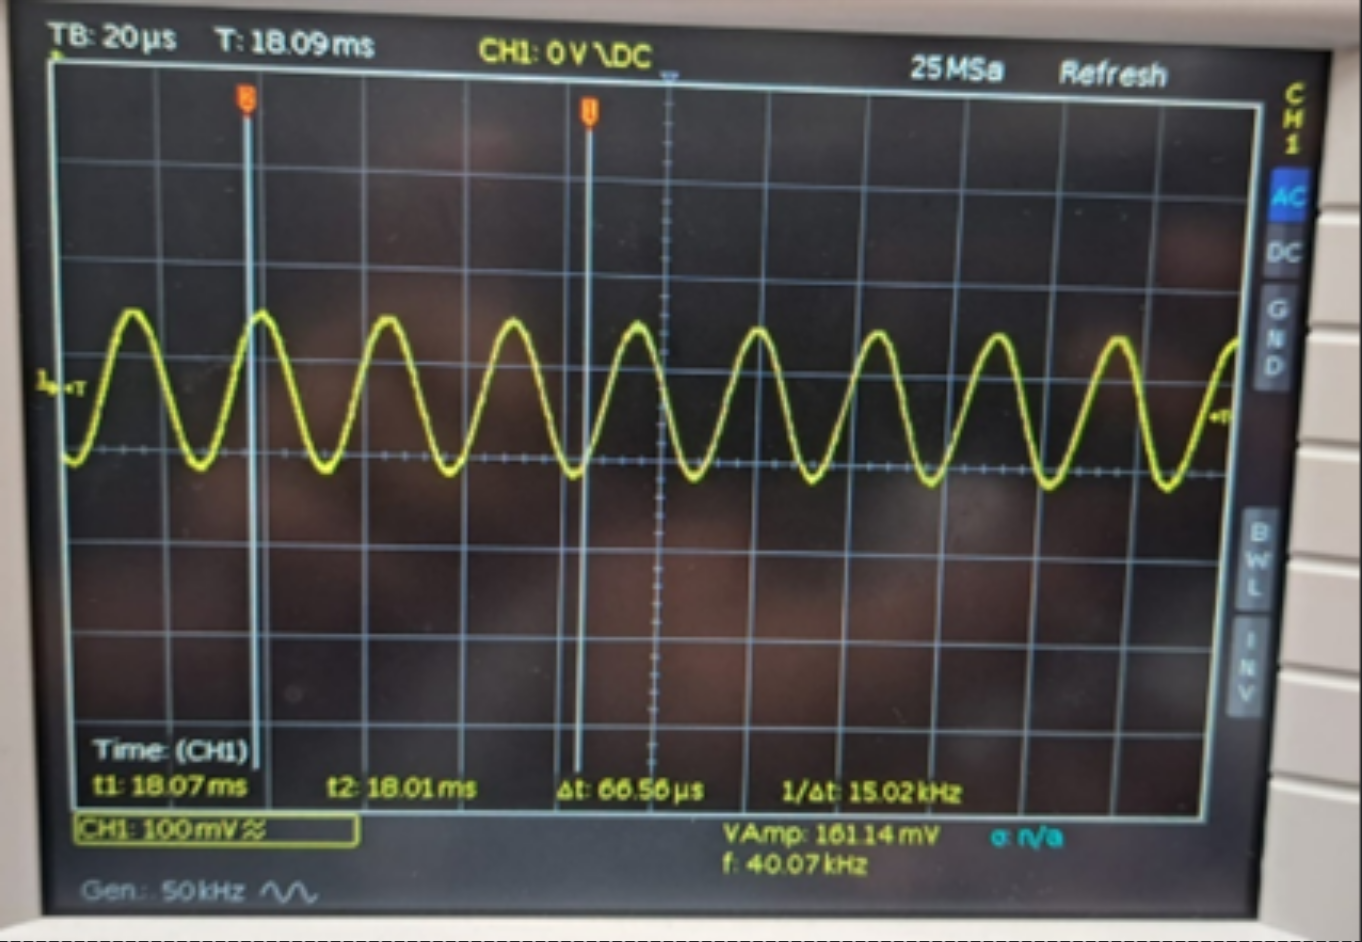
\includegraphics[width=0.8\textwidth]{subpages/images/ultra_oscilloscope_transducer.png}
    \caption{Oscilloscope Waveform of Transducer Signal at Around 160mV Amplitude}
    \label{fig:transducer_waveform}
\end{figure}
To model the sinusoidal waves generated by the sensor, the first section of the overall circuit has been shown below:
\begin{figure}[H]
    \centering
    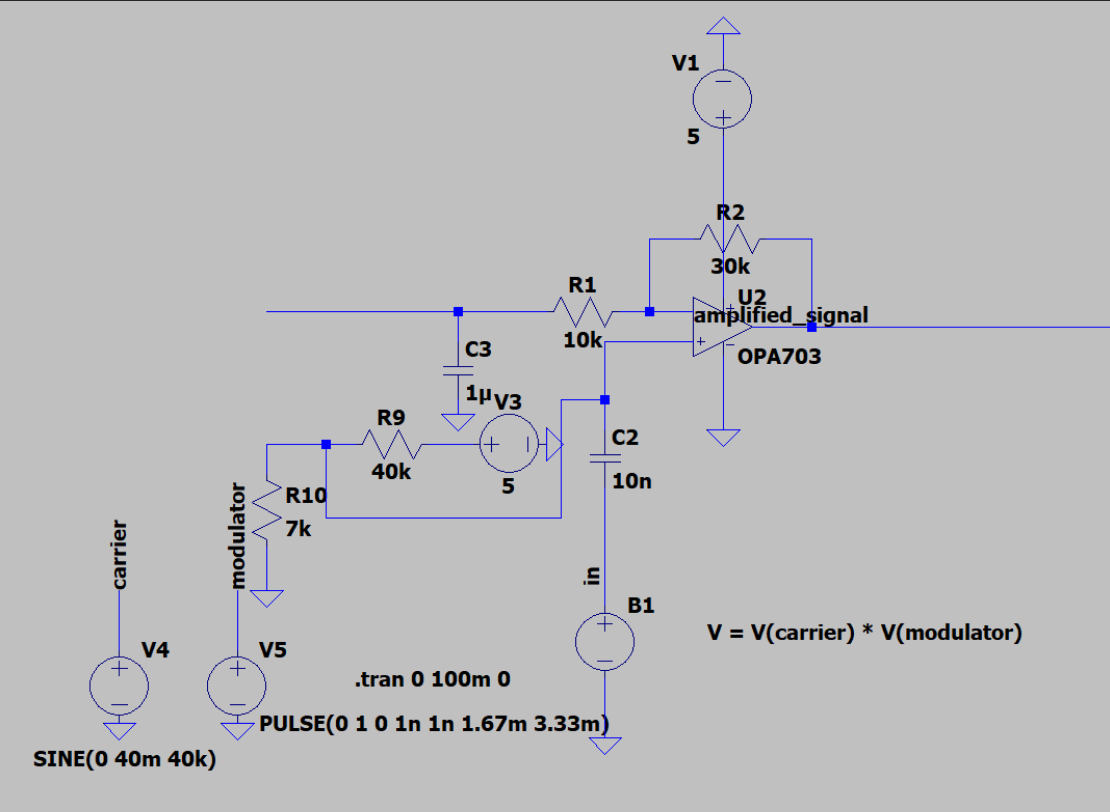
\includegraphics[width=0.8\textwidth]{subpages/images/ultra_circuit_trans_amp.png}
    \caption{Circuit Schematic for the Ultrasound Transducer and Amplifier}
    \label{fig:transducer_amplifier_circuit}
\end{figure}
The behavioural voltage source, B1, is defined by the product of the carrier signal, a sine wave with a frequency of 40kHz and amplitude of 40mV, and a modulated signal, imitating the ASK modulation stated prior. Given a transient simulation running for 100ms on LTspice, the waveform produced the expected output. It should be noted that a 40mV amplitude was used in simulation as an estimate of the amplitude from the transducer.

\begin{figure}[h]
    \centering
    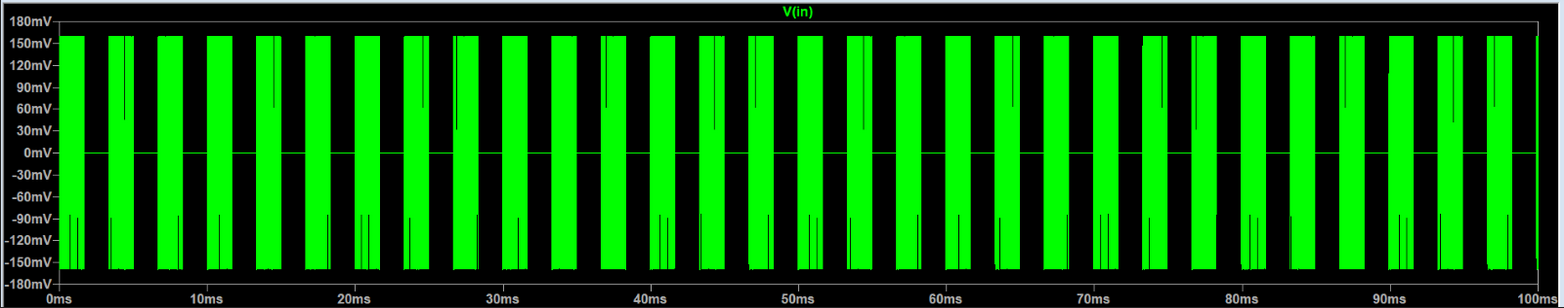
\includegraphics[width=0.8\textwidth]{subpages/images/ultra_bv_output.png}
    \caption{Output Waveform for the Behavioural Voltage Source}
    \label{fig:bv_waveform}
\end{figure}
The amplitude of this signal shown in LTspice is 150mV, this signal is extremely low and thus requires amplification to allow for envelope detection and to act as a binary signal. A large voltage difference is required between the high and low outputs, this cannot be achieved with a 150mV input to a comparator. Therefore, this signal must be amplified. This is done using a non-inverting amplifier.  The non-inverting amplifier was chosen due to having a positive gain as well as having a simple design (Cadence PCB Solutions, 2024).
\begin{figure}[h]
    \centering
    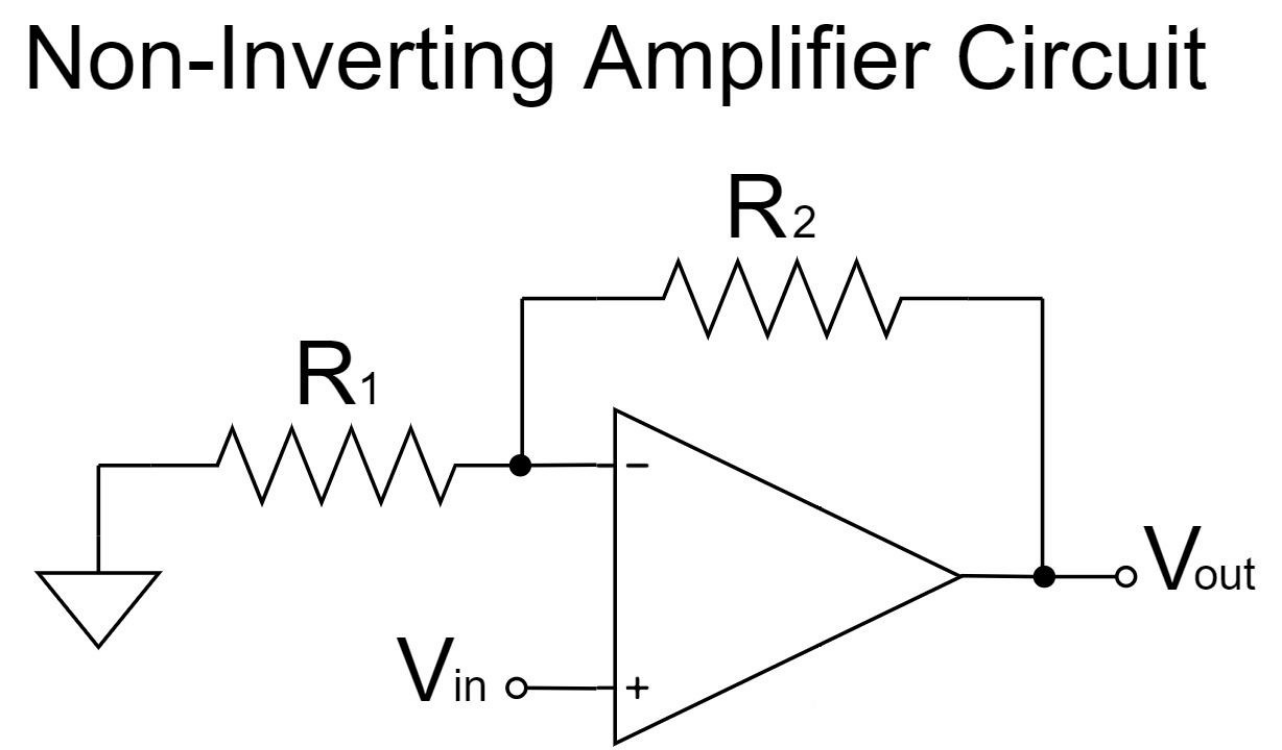
\includegraphics[width=0.8\textwidth]{subpages/images/non_invert_amp.png}
    \caption{Non-Inverting Amplifier Circuit (Spiceman, 2022)}
    \label{fig:non_inverting_amp}
\end{figure}
Given this circuit, the gain of the circuit is given as such: \(1+ \frac{R_f}{R_{In}} \).

A gain of 4 was deemed to give a high enough output to allow for the next stages of the circuit to work effectively. This is achieved with R2 being equal to 30k and R1 being 10k. This produces the desired output shown below. Furthermore, due to the bias signal connected to the non-inverting input of the op-amp, the DC offset is around 750mV, this is much lower when practically built which will be important in the next stage of the circuit.  A key point is that there is no ground in the negative input of the amplifier, ensuring there is no DC offset from it.
\begin{figure}[h]
    \centering
    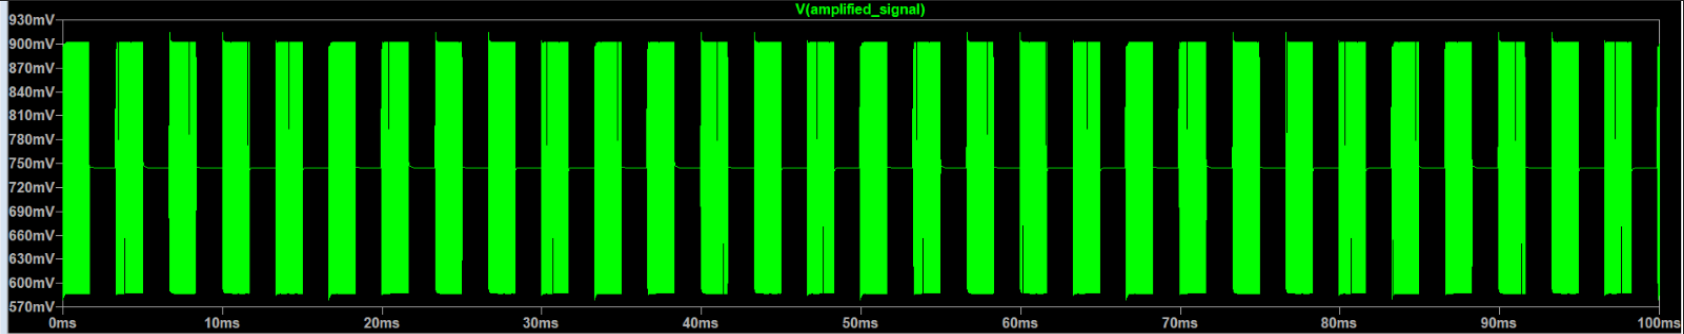
\includegraphics[width=0.8\textwidth]{subpages/images/ultra_output_amplified.png}
    \caption{Output Waveform for the Amplified Signal}
    \label{fig:amplified_output}
\end{figure}

Researching components suggests that an array of op-amps will be required in this project rather than mimicking op-amps from previous sections for the sake of simplicity. In this case, the OPA703 op-amp was used due to its high slew rate of 0.6V/µs, thus allowing for a quick response to the change in signals [5]. Moreover, it allowed for a rail-to-rail input/output thus allowing for the power rails to be 5V and 0V. This also allows for the output waveform to stay positive due to the ground-referenced supply to the negative power rail of the op-amp.

Building further, the low quiescent current of 160µA makes this op-amp suitable for relatively low-power applications such as a duck detection system as the electronic architecture of the work is not overly power-demanding. With an input voltage noise density of \(45nV/\quad{Hz}\) and low offset voltage, the OPA703 limits noise interference, which is crucial for detecting small-amplitude signals from the transducer. Therefore, this greatly enhances the signal-to-noise ratio during amplification. The additional presence of high common-mode rejection ratio of 90dB ensures that common-mode noise is rejected.
\begin{figure}[h]
    \centering
    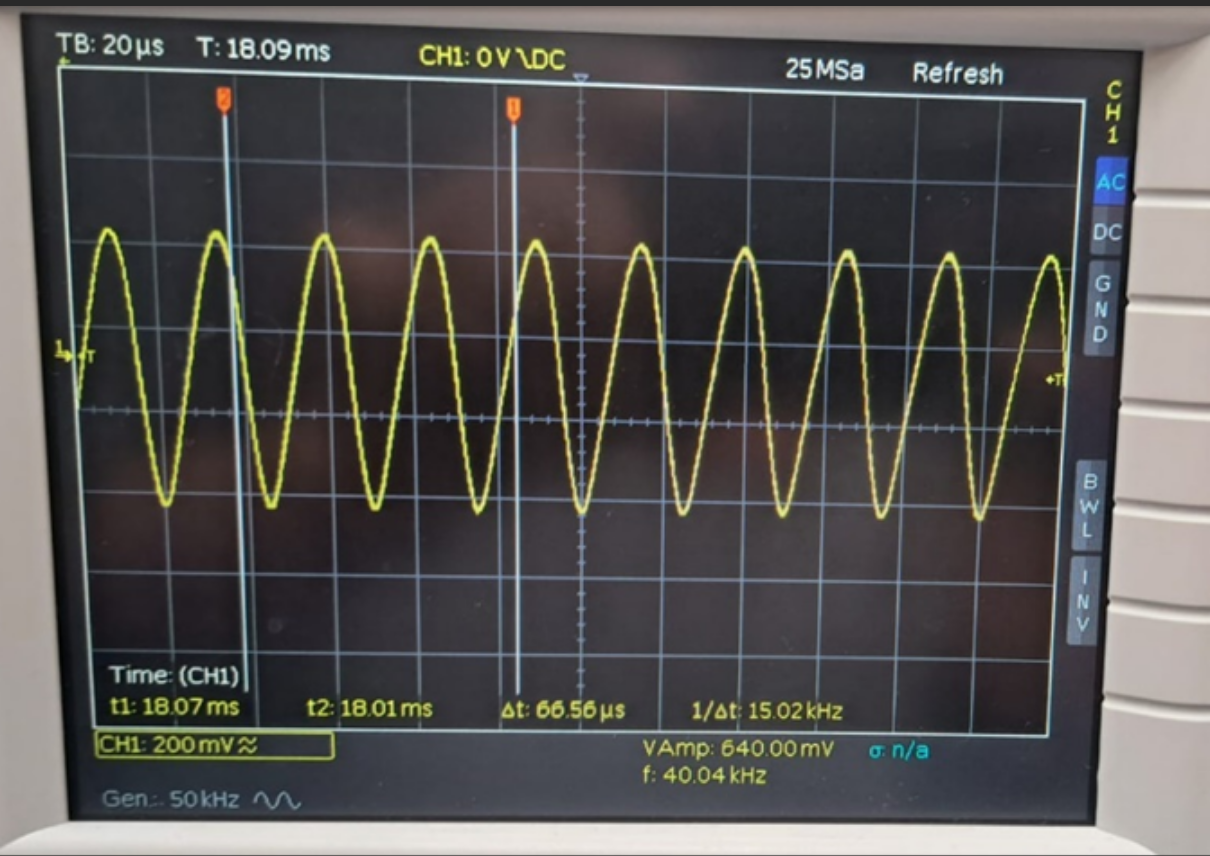
\includegraphics[width=0.8\textwidth]{subpages/images/ultra_4_gain.png}
    \caption{Waveform of 4x Amplified Ultrasonic Signal}
    \label{fig:waveform_4x_gain}
\end{figure}

\section{Envelope detector}
The envelope detector demodulates the signal from the ultrasound transducer, involving the extraction of a desired signal from a modulated carrier signal at the receiver end.
\begin{figure}[h]
    \centering
    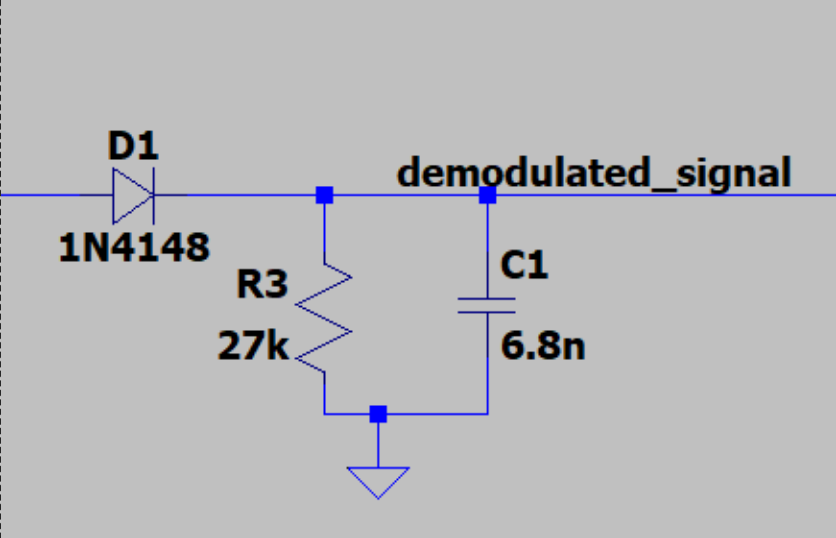
\includegraphics[width=0.8\textwidth]{subpages/images/ultra_envelope.png}
    \caption{Circuit Schematic for the Envelope Detector}
    \label{fig:envelope_detector}
\end{figure}
The diode is used to reduce the amplitude of oscillations due to the op-amp thus demodulating the signal [6]. The diode chosen was the 1N4148 for its fast-switching and cheap price7. In the section prior, it was mentioned that a low DC offset was key for the next section. This is because due to the ASK modulation, when a low input was given, a high DC offset would cause the diode to remain on and thus there would be no change in a logic 1 and 0 input in the final output. The expected output can be seen in the figure below:
\begin{figure}[h]
    \centering
    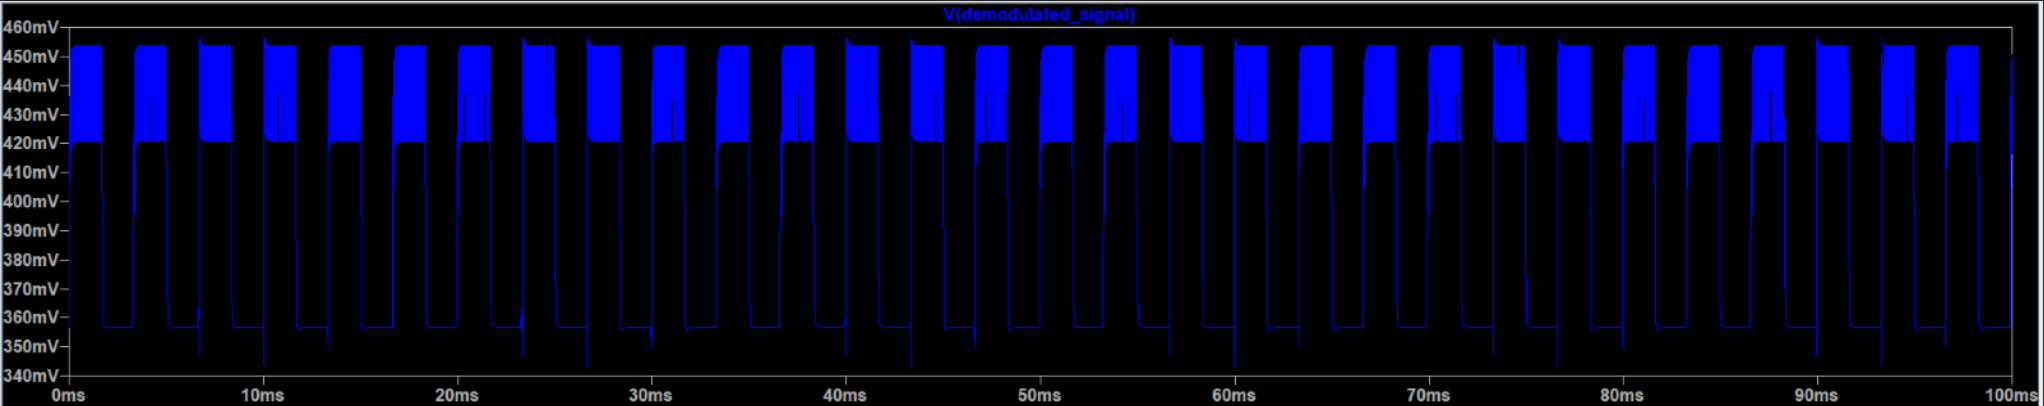
\includegraphics[width=0.8\textwidth]{subpages/images/ultra_output_demodulated.png}
    \caption{Output Waveform for the Demodulated Signal}
    \label{fig:demodulated_waveform}
\end{figure}

The low pass filter after the diode is used to ensure that the carrier frequency is filtered out. Moreover, as the signals of the duck have a frequency of 600Hz, given by the 600 bits per second stated in the introduction, this frequency must be passed through the filter. Therefore, the corner frequency of this filter must be significantly under 40kHz and greater than 600Hz to ensure that all required signals are picked up accounting for any fluctuations from the stated frequencies. Therefore, the corner frequency was chosen to be 900Hz. The equation used: \(f_c = \frac{1}{2\pi RC}\)

Given that: RC must be equal to approximately 0.184ms; and the available components in the lab, the following values of R and C in figure 29 were chosen. This gave a corner frequency of 867Hz shown to be achieved through AC analysis on LTspice.
\begin{figure}[H]
    \centering
    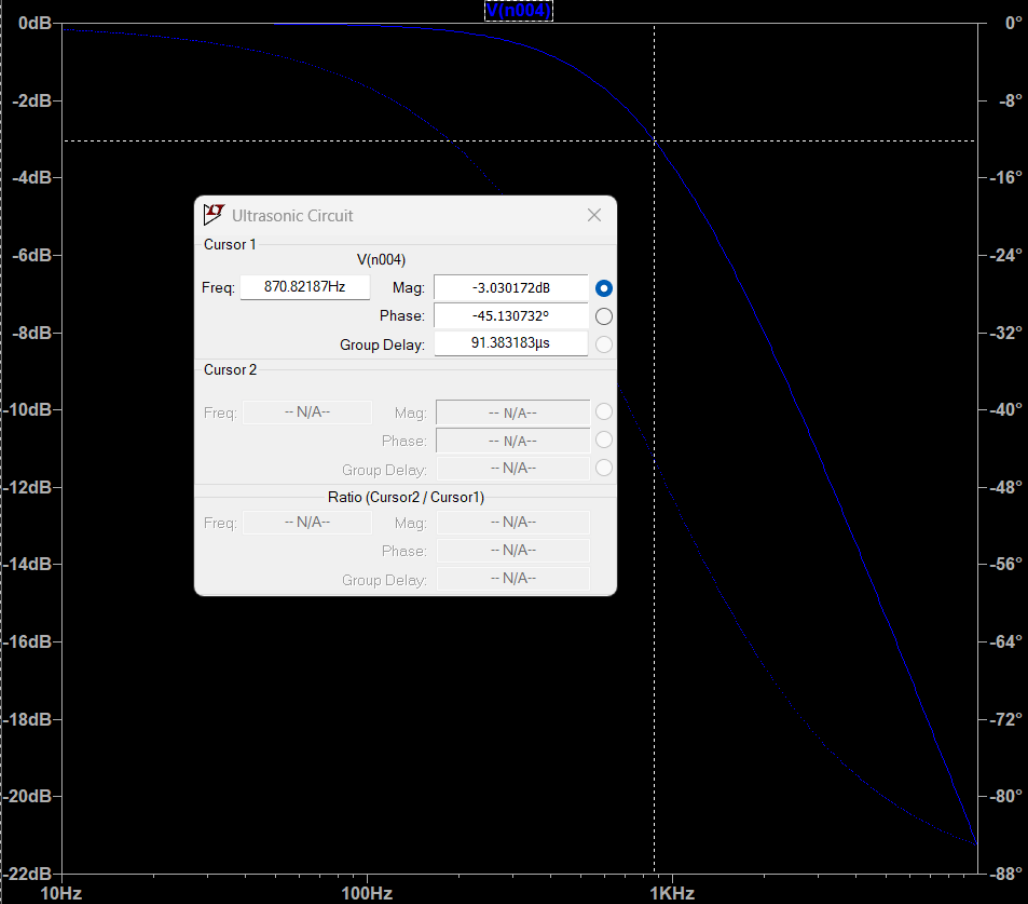
\includegraphics[width=0.45\textwidth]{subpages/images/ultra_lp.png}
    \caption{Magnitude Response for the Low-Pass Filter With its Corner Frequency}
    \label{fig:mag_response_lp}
\end{figure}

\section{Comparator}
A Schmitt trigger is used as a comparator to convert the demodulated analogue signal from the envelope detector to a digital signal by giving a high output when the voltage reaches a certain threshold and giving an output of zero volts otherwise [8].
\begin{figure}[h]
    \centering
    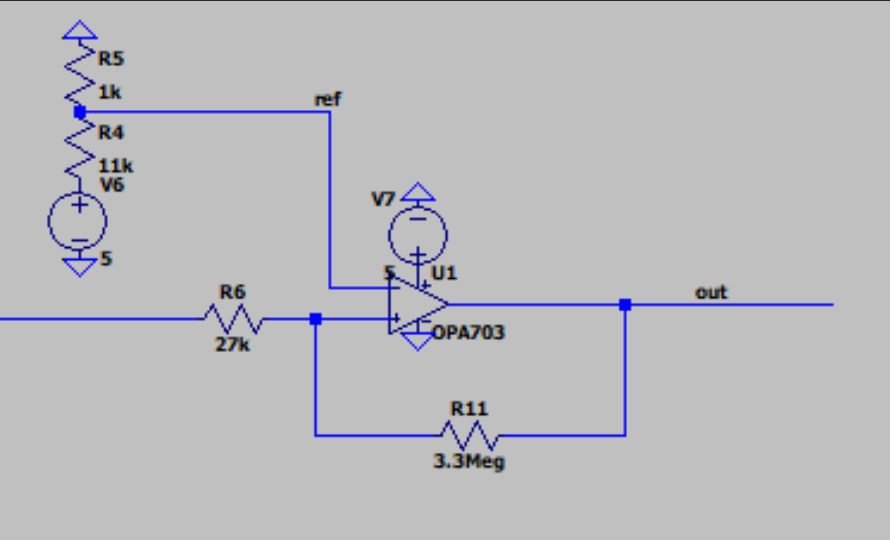
\includegraphics[width=0.8\textwidth]{subpages/images/ultra_comparator.png}
    \caption{Circuit Schematic for the Comparator Circuit}
    \label{fig:comparator}
\end{figure}

The voltage divider is given by the V6, R4 and R5. This provides the reference voltage for the comparator connected at V-. The reference voltage, Vref, is given as such: \(V_{ref}  = \frac{R_5}{R_5 + R_6}V_{CC}\)

Given Vcc = 5V, the resister values in figure 32 were chosen as they gave the most accurate signals as well as the sharpest transitions between the high and low states; a high resistance for R4 would cause a slower transition and a lower resistance would cause chattering, multiple rapid transitions [9], in the output. This gives the reference voltage of 412mV shown below.
A Schmitt trigger is used as a comparator to convert the demodulated analogue signal from the envelope detector to a digital signal by giving a high output when the voltage reaches a certain threshold and giving an output of zero volts otherwise [8].
\begin{figure}[h]
    \centering
    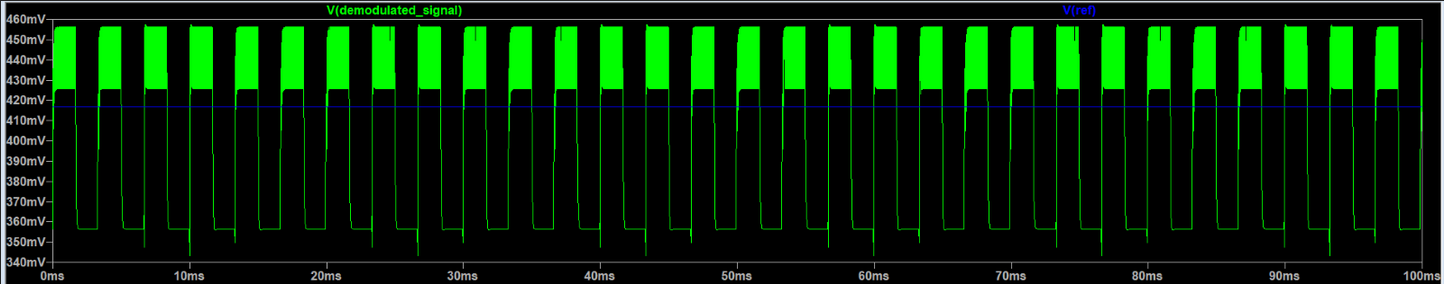
\includegraphics[width=0.8\textwidth]{subpages/images/ultra_reference_out.png}
    \caption{Output Waveform for the Reference Voltage Relative to the Demodulated Signal}
    \label{fig:reference_output}
\end{figure}

Originally, an MP6561 output comparator was going to be used [10], however due to these comparators being surface mount components exclusively, this comparator was not suitable due to issues with prototyping and other sections required for the overall project11 i.e. it would make it more difficult to implement with the entire rover.

Therefore, the OPA703 op-amp is used here to function as a comparator. Although it has a slower slew rate than the MP6561, this should not be an issue due to the slow input transitions compared to this rate. As an op-amp is used rather than a comparator, the Schmitt trigger is used to reduce chattering when built practically. This is because there is greater hysteresis in this design in comparison to using a comparator circuit.
\begin{figure}[h]
    \centering
    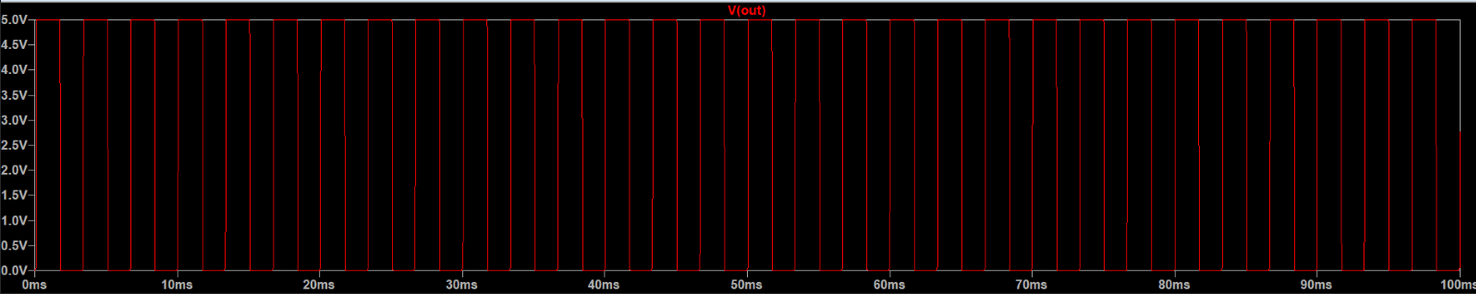
\includegraphics[width=0.8\textwidth]{subpages/images/ultra_binary_out.png}
    \caption{Output Waveform of the Binary Signal}
    \label{fig:binary_signal}
\end{figure}
\begin{figure}[h]
    \centering
    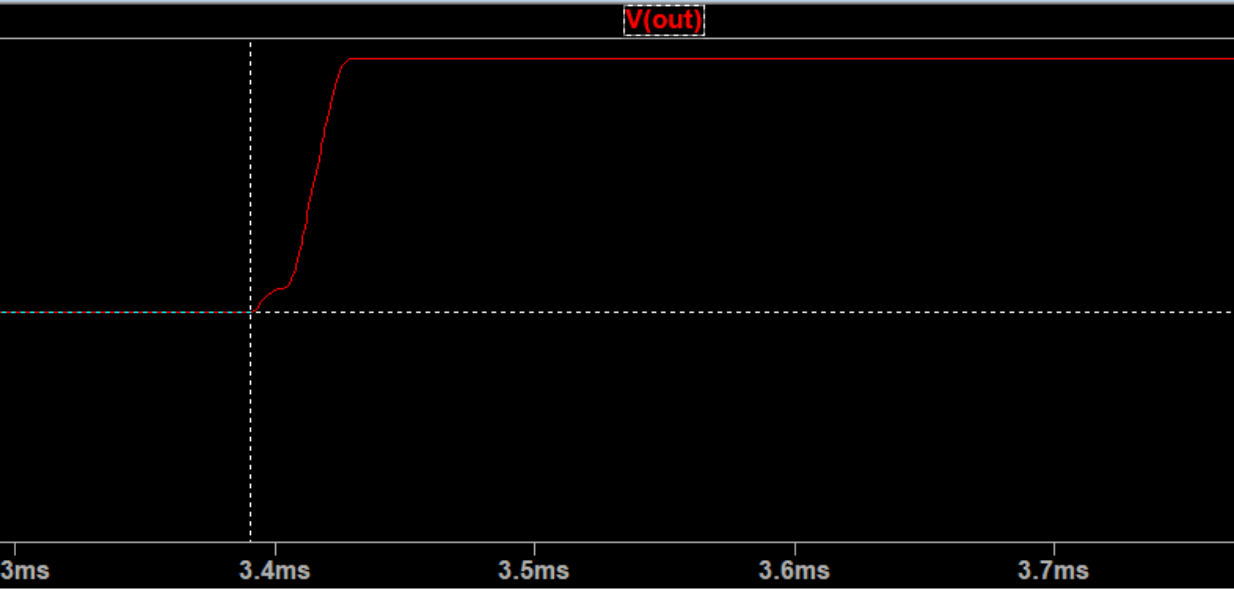
\includegraphics[width=0.8\textwidth]{subpages/images/ultra_binary_transition.png}
    \caption{Output Waveform of the Binary Signal at the Transition. The transition Time via LTspice was 37$\mu$s}
    \label{fig:binary_transition}
\end{figure}

The overall circuit was then constructed and assessed to give binary outputs.
\begin{figure}[H]
    \centering
    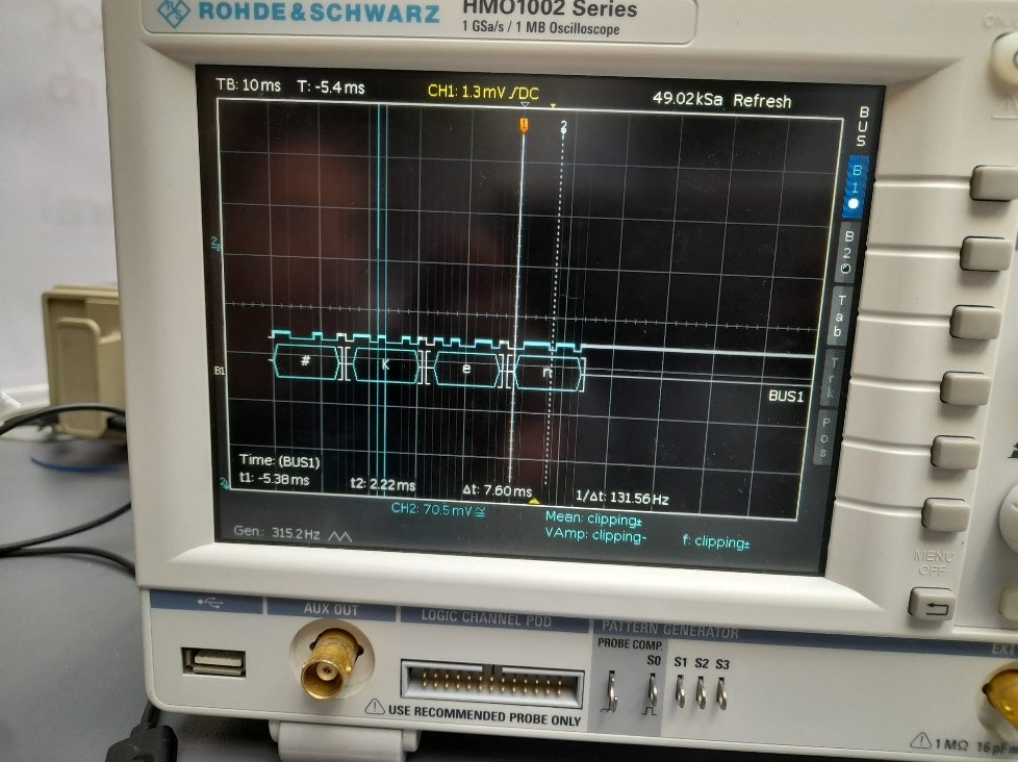
\includegraphics[width=0.6\textwidth]{subpages/images/ultra_out.png}
    \caption{Oscilloscope Waveform of the Output Binary Signal}
    \label{fig:binary_transition}
\end{figure}
In conclusion, the ultrasonic detection circuit produces the binary output shown in figure 5.17. Future improvements to this design may include higher gain in the amplifier circuit allowing for detection at a further distance and increased hysteresis in the comparator reducing the chattering in the final output. A key concept in building this circuit was demodulation. This continued to be integral in signal analyses as seen in the construction of the radio detectors.

\chapter{Radio Detection}
\section{Initial Ideas}

While species analysis via IR detection relied upon phototransistors and optical filtering, radio signal detection introduces distinct challenges in circuit design and frequency testing. For our desired species – Gribbit and Zapple, our goal was to build a circuit capable of:

\begin{enumerate}
    \item Capturing AM-modulated radio signals.
    \item Selecting the correct carrier frequency (89kHz).
    \item Demodulating the signal to extract low-frequency data.
    \item Amplifying the signal to a detectable level.
\end{enumerate}

While the brief proposed using a tuned coil antenna, we opted for a standard inductor based on predictable characteristics and ease of integration. The table below compares both options:

\begin{table}[H]
    \centering
    \begin{tabular}{|l|l|l|}
        \hline
        \textbf{Inductor Type}     & \textbf{Tuned-Coil Antenna}    & \textbf{Standard Inductor} \\
        \hline
        Primary Role               & RF signal Reception            & Energy Storage             \\
        Ease of Use/Predictability & Requires Tuning                & No tuning required         \\
        Q Factor                   & High (Narrow Bandwidth)        & Moderate to High           \\
        Frequency Range            & Narrow                         & Broad                      \\
        Impedance Matching         & Must match RF system impedance & No need to match           \\
        Size                       & Larger                         & Compact                    \\
        Parasitic Effects          & High                           & Low                        \\
        \hline
    \end{tabular}
    \caption{Comparison of Inductor Types}
    \label{tab:inductors}
\end{table}

\section{Circuit Design}

The carrier frequency of 89kHz is isolated using a parallel LC resonant circuit. The resonance condition is given by the following formula:
\[
    f_0 = \frac{1}{2\pi\sqrt{RC}} \quad \rightarrow \quad LC = \frac{1}{(2\pi f_0)^2}
\]
For a \( f_0 = 89000\,\text{Hz} \), this gives:
\[
    LC \approx 3.2 \cdot 10^{-12}
\]

To achieve a narrower, more selective bandwidth, we require a higher quality factor which varies inversely with capacitance. We start with a 68pF capacitor, which implies the LC filter will require roughly 47mH of inductance to resonate at the carrier frequency. These values define the first stage of the filter circuit.
\begin{figure}[H]
    \centering
    \includegraphics[width=0.8\textwidth]{subpages/images/radio_LTspice_rc_circuit.png}
    \caption{RC Circuit in LTspice}
    \label{fig:rc_circuit}
\end{figure}

The LTspice simulation used an AC sweep to verify resonance. A sharp peak at ~89kHz confirmed accurate tuning and validated the LC component selection. However, in the grand scheme, the design revolves around a different source - the current was selected a simple means to analyse resonance.
\begin{figure}[H]
    \centering
    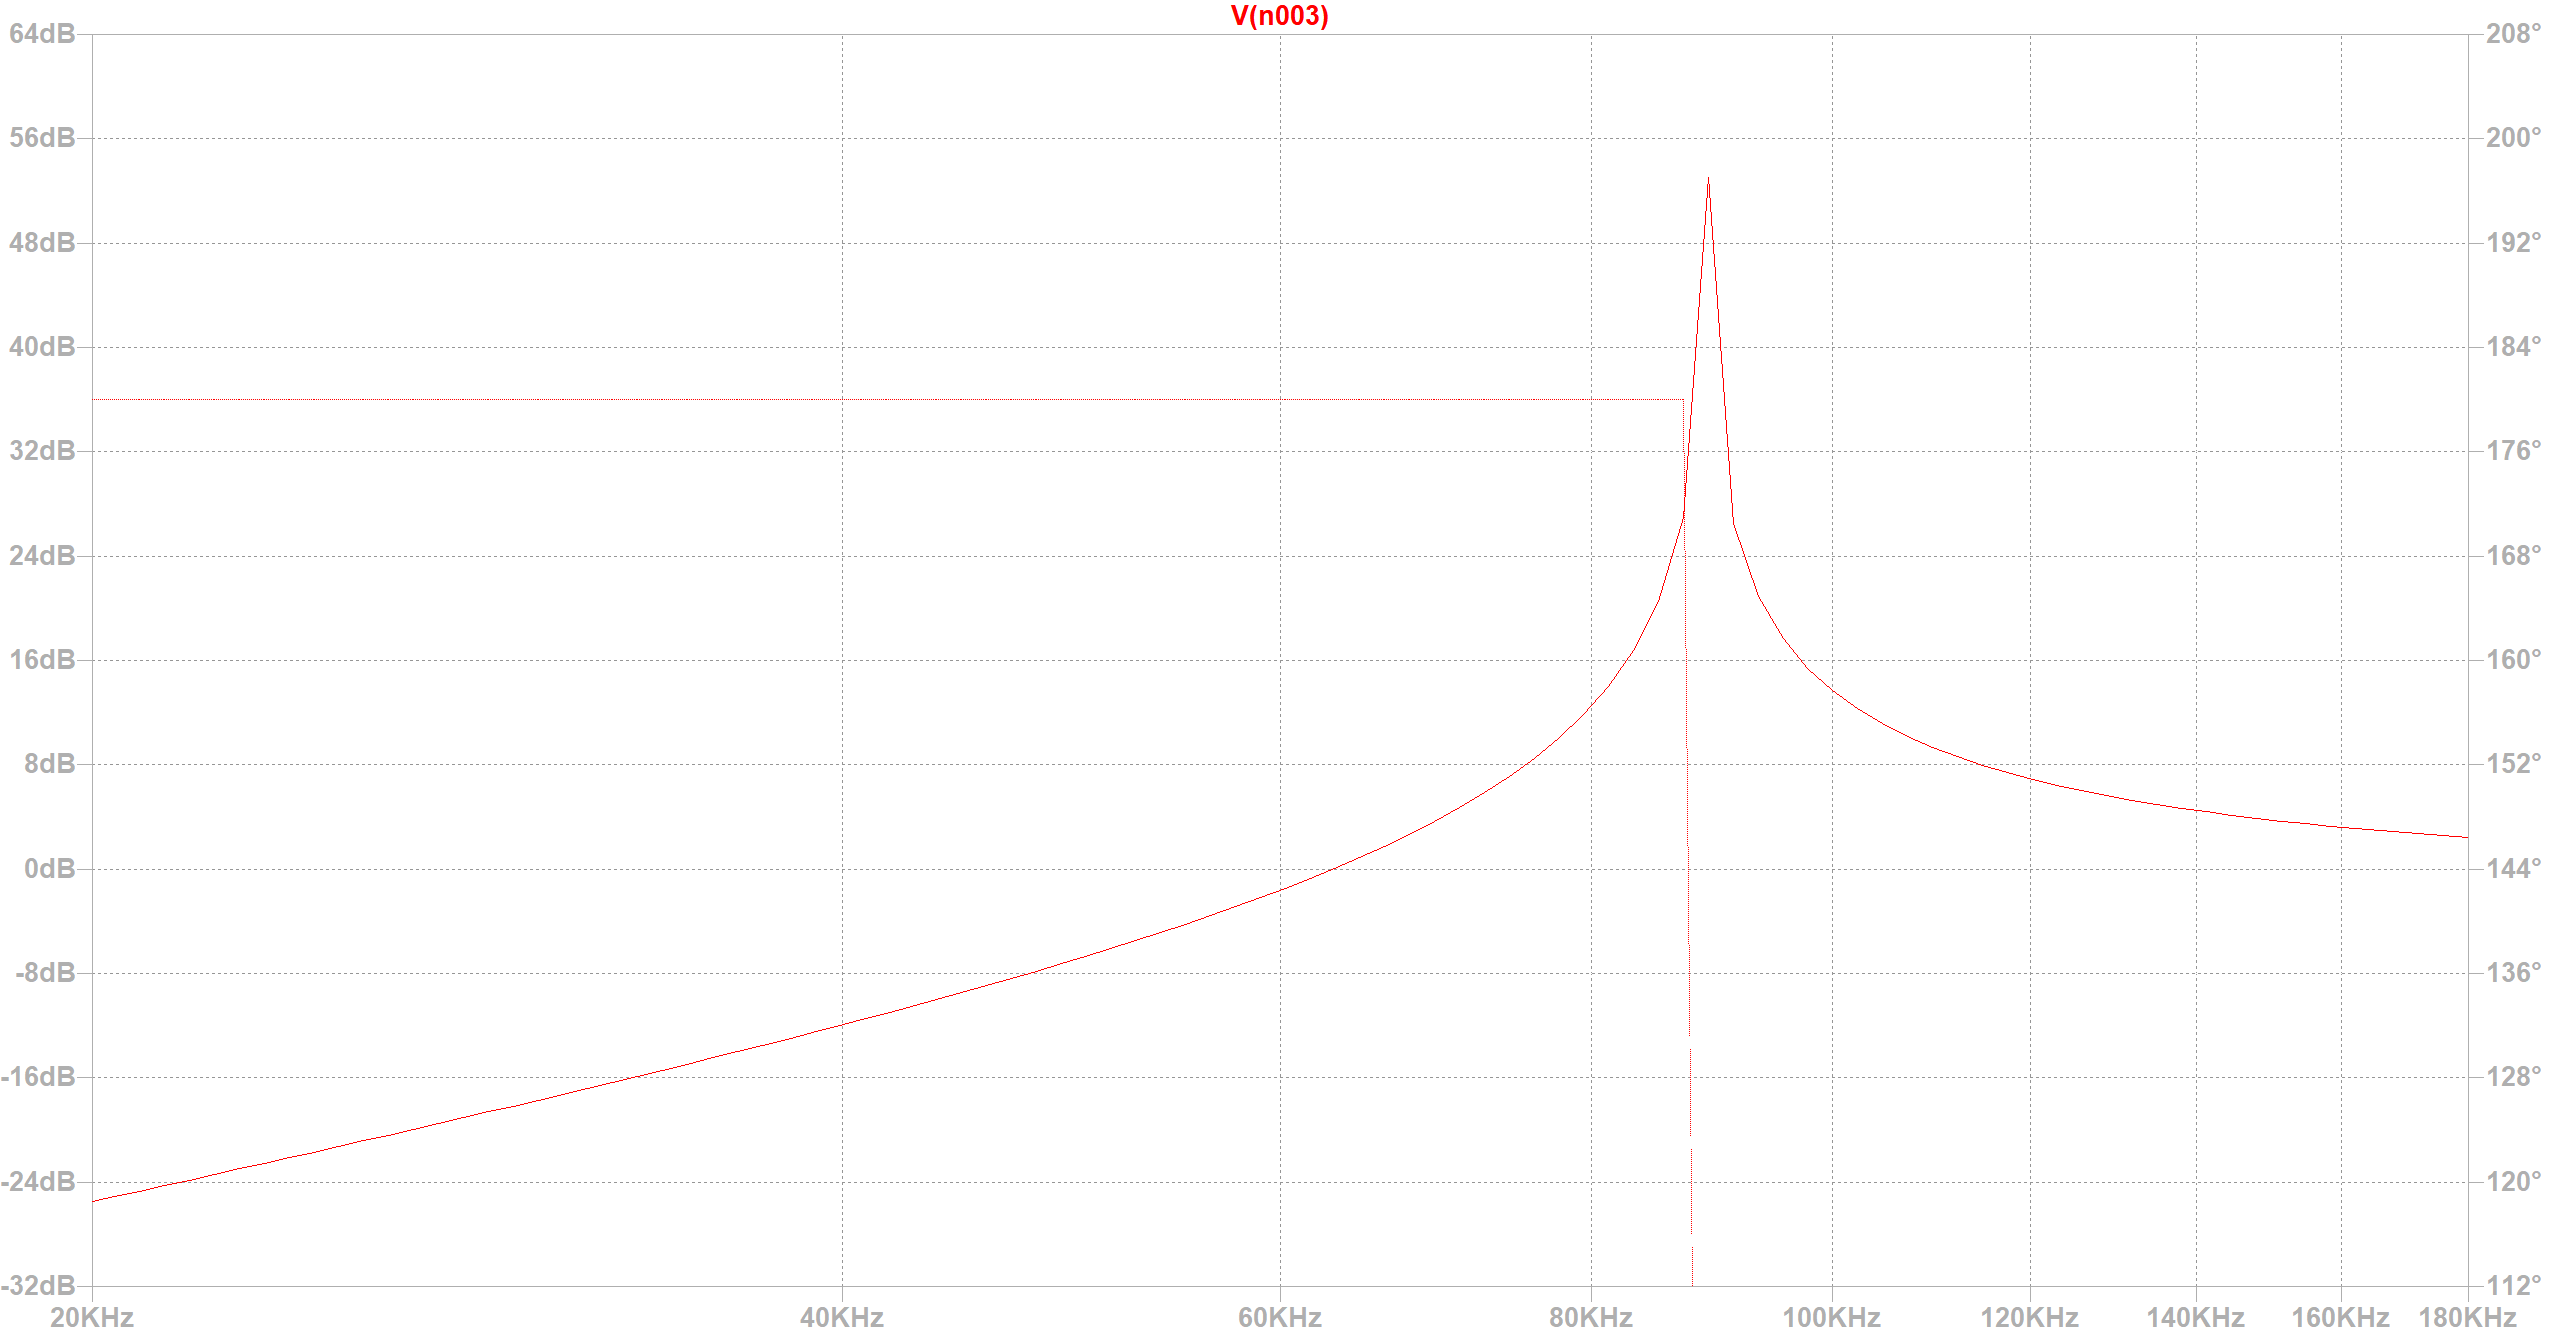
\includegraphics[width=0.8\textwidth]{subpages/images/radio_ac_waveform.png}
    \caption{AC Waveform Showing Resonance}
    \label{fig:ac_waveform}
\end{figure}

\subsubsection{Signal Modelling}

A behavioural voltage source: \( V=(1+0.5\cdot\sin(2\pi\cdot100\cdot\text{time})) \cdot \sin(2\pi\cdot89k\cdot\text{time}) \) was selected to simulate an actual received radio signal, for the following reasons:

\begin{itemize}
    \item The 89kHz carrier is represented by the outer sine function.
    \item The 100Hz message frequency, in the inner sine function, modulates the amplitude.
    \item The modulation depth ensures the signal swings between 0.5V and 1.5V, creating a clear envelope for detection.
\end{itemize}

\begin{figure}[H]
    \centering
    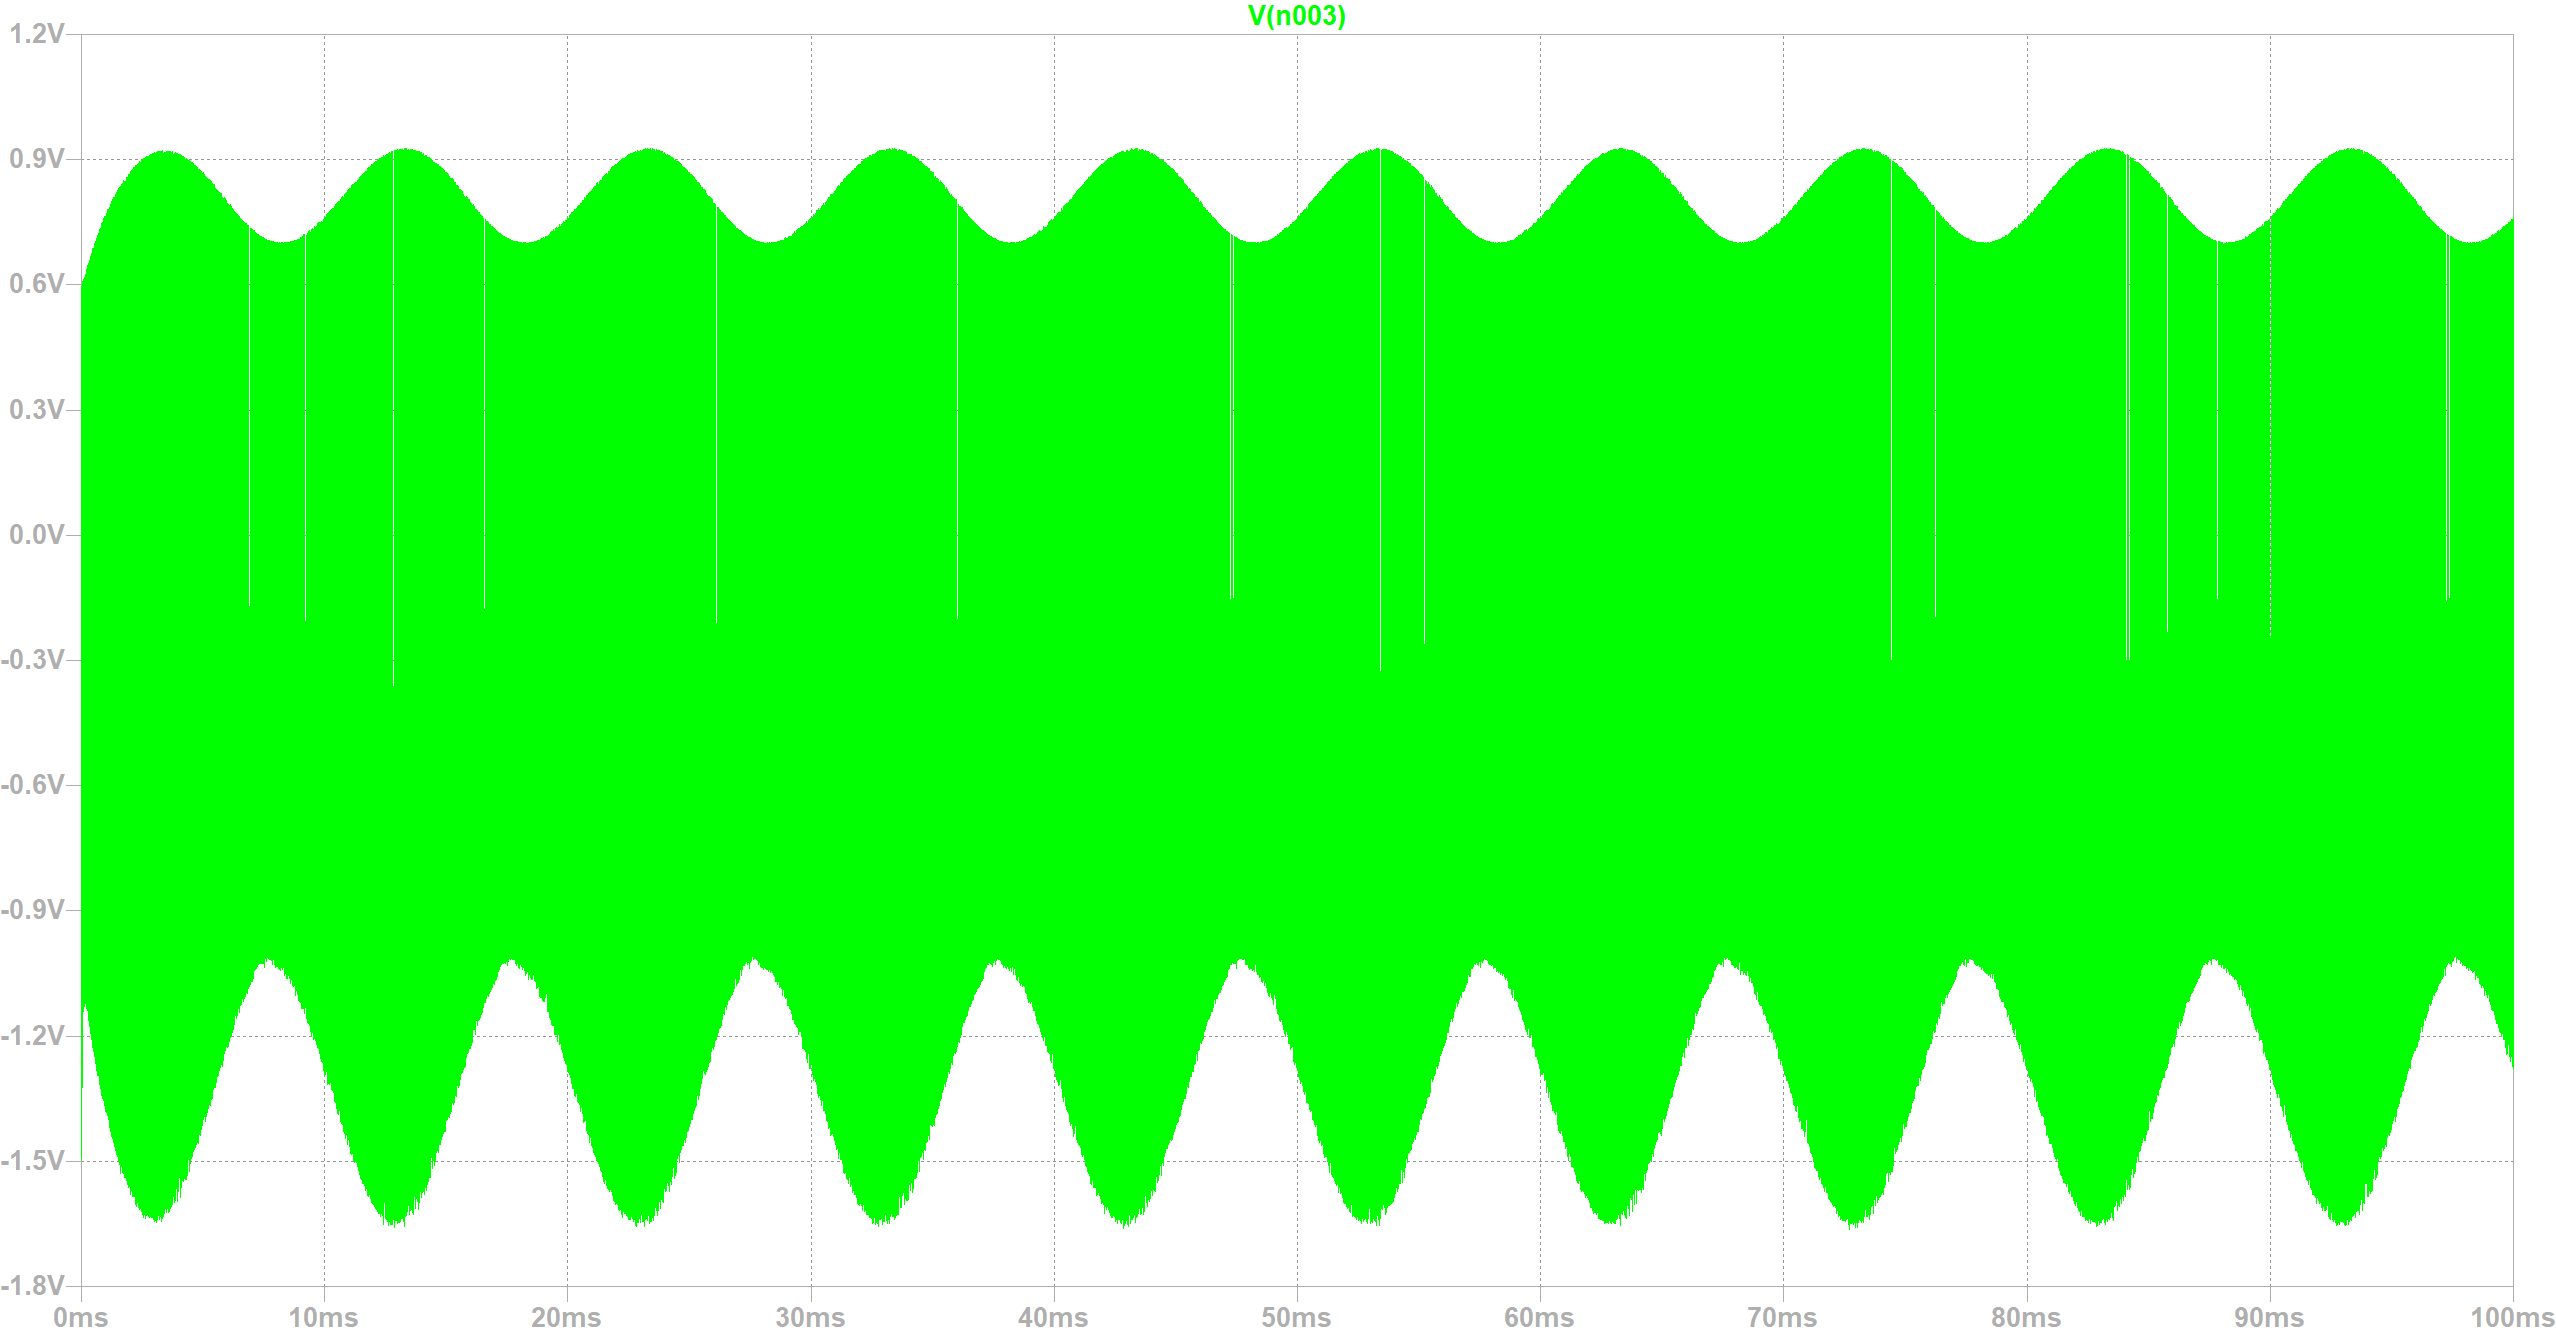
\includegraphics[width=0.8\textwidth]{subpages/images/radio_am_envelope_signal.png}
    \caption{An AM Envelope Signal}
    \label{fig:am_envelope}
\end{figure}

\subsubsection{Demodulation}

We now have the carrier frequency selected and now require the demodulation process using an envelope detector. Demodulation involves extracting a targeted information signal from a carrier signal once it has reached the receiver. Meanwhile, an envelope detector is a specific type of demodulator which serves the purpose of taking a high-frequency signal as input and extracting the varying amplitudes, which outputs the "outline" of the original amplitude modulation signal.

\begin{figure}[H]
    \centering
    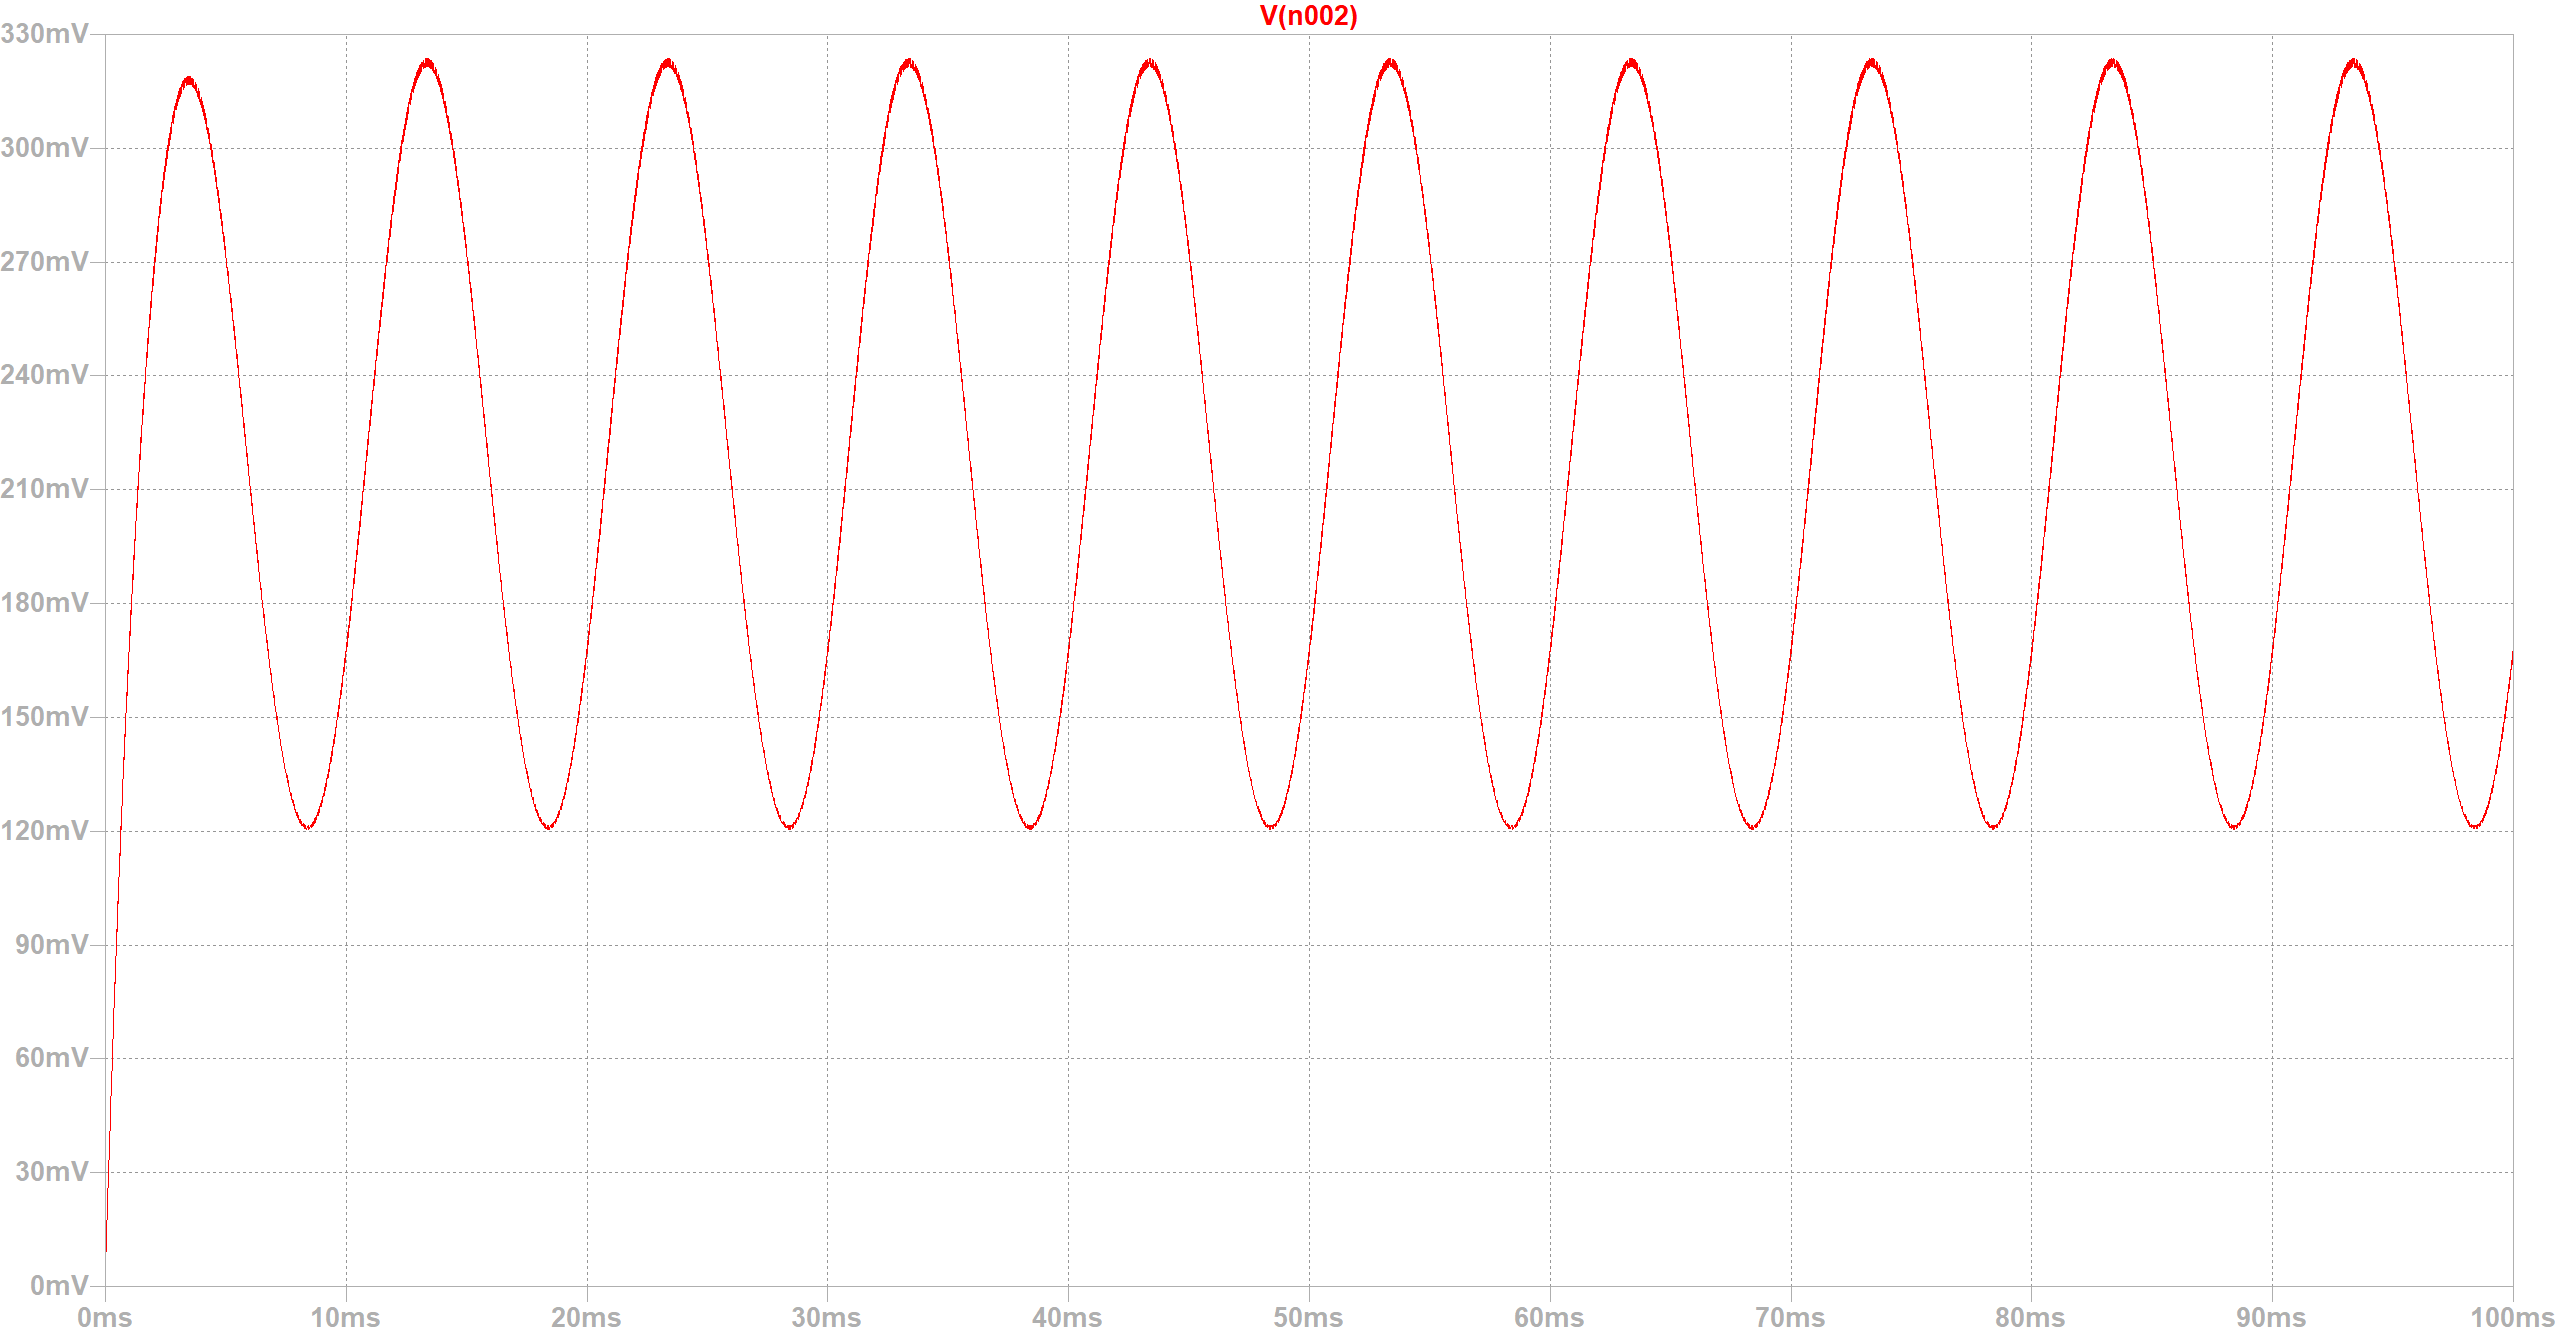
\includegraphics[width=0.8\textwidth]{subpages/images/radio_envelope_output.png}
    \caption{Output of the Envelope Detector }
    \label{fig:envelope_output}
\end{figure}

To extract the low-frequency data (e.g. 100Hz or 150Hz depending on species), the envelope detector was implemented using a diode, resistor, and capacitor:

\begin{itemize}
    \item The diode rectifies the signal.
    \item The RC filter smooths out the high-frequency carrier.
    \item The resulting waveform reflects the amplitude variation, i.e., the message signal.
\end{itemize}

This simulation output confirmed the demodulation stage successfully filtered out the carrier, leaving behind a readable low-frequency waveform.

\subsubsection{Signal Amplification}

Finally, the LTspice circuit concerns itself with amplifying the weak, raw signal stemming from the demodulation process. The envelope detector relies upon an imperfect diode which will trace out the desired waveform shape but fails to boost the power of the wave, rendering it faint for detection. Therefore, it was passed through a two-stage non-inverting op-amp amplifier. Each stage has a gain of:

\[
    1 + \frac{R_f}{R_{\text{in}}} = 1 + \frac{20k\Omega}{1k\Omega} = 21
\]

This leads to a total gain of \( 21 \cdot 21 = 441 \). We use two stages to avoid clipping or distortion from high single-stage gain, and bandwidth reduction or instability in the amplifier. A voltage follower precedes the amplifier to buffer the signal and ensure low output impedance from the envelope detector.

\subsubsection{Building and Testing}

The final circuit was built in stages, each validated independently:

\begin{enumerate}
    \item  Envelope Detection - verified with LTspice and matched our theoretical expectations. The diode and RC values didn't need tuning for a smooth envelope at 100-150Hz range as the theoretical values proved ample enough.
    \item Amplification - we first breadboarded and tested with synthetic input. The two-stage gain provided a clean, amplified waveform observable on an oscilloscope.
    \item Full System Integration - the final circuit captures the AM-modulated signal, filters and amplifies it for reliable species detection via \texttt{analogRead} in the Arduino code. It can distinguish between Gribbit (100Hz) and Zapple (150Hz) based on the output frequency. Refer to Chapter 8 for more detail on the code.
\end{enumerate}

\begin{figure}[H]
    \centering
    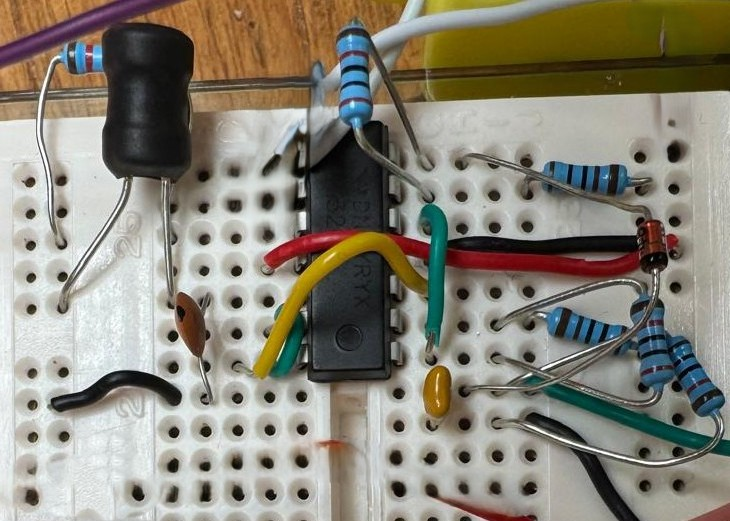
\includegraphics[width=0.8\textwidth]{subpages/images/radio_circuit.jpg}
    \caption{Final Built Circuit}
    \label{fig:radio_circuit}
\end{figure}

While our study on radio waves revealed the duck's frequencies through demodulation, this does not reveal the full picture. Beyond analysis of waves, there are polarities hidden which must be acknowledged. To ensure no duck is left unidentified, the focus now switches to the magnetic detection system.


\chapter{Magnetic Detection}
\section{Initial Ideas}
The initial approach to the magnetism task focused on reliably detecting the static magnetic fields emitted by the ducks to identify species through their distinct polarities. Early testing with the DRV5053 Hall sensor revealed significant challenges in achieving consistent detection. When the sensor was placed in direct contact with the duck's head, the output voltages correctly indicated the magnetic polarity. However, at even small distances of just a few millimetres, the signal strength dropped dramatically, making it impossible to determine the field direction reliably.

These preliminary results made it clear that additional signal conditioning would be necessary for practical implementation. The key requirements emerged as amplifying the weak magnetic signals to extend the detection range while implementing proper filtering to stabilize the output against noise. The trade-offs between sensitivity, noise immunity, and physical positioning became the primary focus for further development.

\section{Hall Effect Sensor}
The Hall effect sensor operates on the principle of detecting magnetic fields through the deflection of charge carriers in a semiconductor material. When exposed to a magnetic field perpendicular to its sensing surface, the sensor generates a voltage proportional to the field strength. Our initial testing with the DRV5053 sensor revealed several important characteristics about its behaviour in our specific application. With the sensor placed directly against the duck's head, the output voltage clearly indicated the magnetic polarity. However, this reliable detection only occurred at impractically close distances.

\section{DRV5053 Hall Sensor Analysis}
\begin{table}[H]
    \centering
    \begin{tabular}{|p{4cm}|p{10cm}|}
        \hline
        \textbf{Sensor Characteristic} & \textbf{Analysis}                                                                                                                                                                                                                                                                                                                     \\
        \hline
        Field and Polarity Detection   & Detects static magnetic fields from the ducks; distinguishes magnetic fields based on voltage increases/decreases from the 1.0V baseline. Sensor response is maximized when the magnetic field is aligned perpendicular to the sensor face, adhering to the Lorentz force principle (\( F = B \cdot I \cdot L \cdot \sin(\theta) \)). \\
        \hline
        Output Type                    & Linear voltage (0.2V to 1.8V) centred around 1.0V with no magnetic field.                                                                                                                                                                                                                                                             \\
        \hline
        Temperature Stability          & Maintains ±10\% sensitivity over –40°C to 125°C - stable for varying environments.                                                                                                                                                                                                                                                    \\
        \hline
        Noise Level                    & As low as 5mV\textsubscript{pp} but filtering may be required to ensure signals are stable under weaker magnetic fields.                                                                                                                                                                                                              \\
        \hline
    \end{tabular}
    \caption{DRV5053 Hall Sensor Characteristics}
    \label{tab:sensor_characteristics}
\end{table}

The LTspice ideal model of the DRV5053 (Figure 7.1) produced a clean and stable output waveform when modelled with ideal conditions, showing distinct voltage levels for north and south pole detection. The simulated output of the DRV5053 LTspice model (see Figure 7.2) perfectly matched our microcontroller's analogue input specifications with its 0.2V to 1.8V output range. However, testing exposed several significant limitations that needed addressing. The most critical issue became apparent when attempting to detect fields at even modest distances of just a few centimetres – the output signal weakened dramatically, making reliable polarity detection impossible. The sensor's sensitivity proved insufficient for our required detection range, as the magnetic field strength diminished rapidly with distance according to the inverse-square law.
\begin{figure}[H]
    \centering
    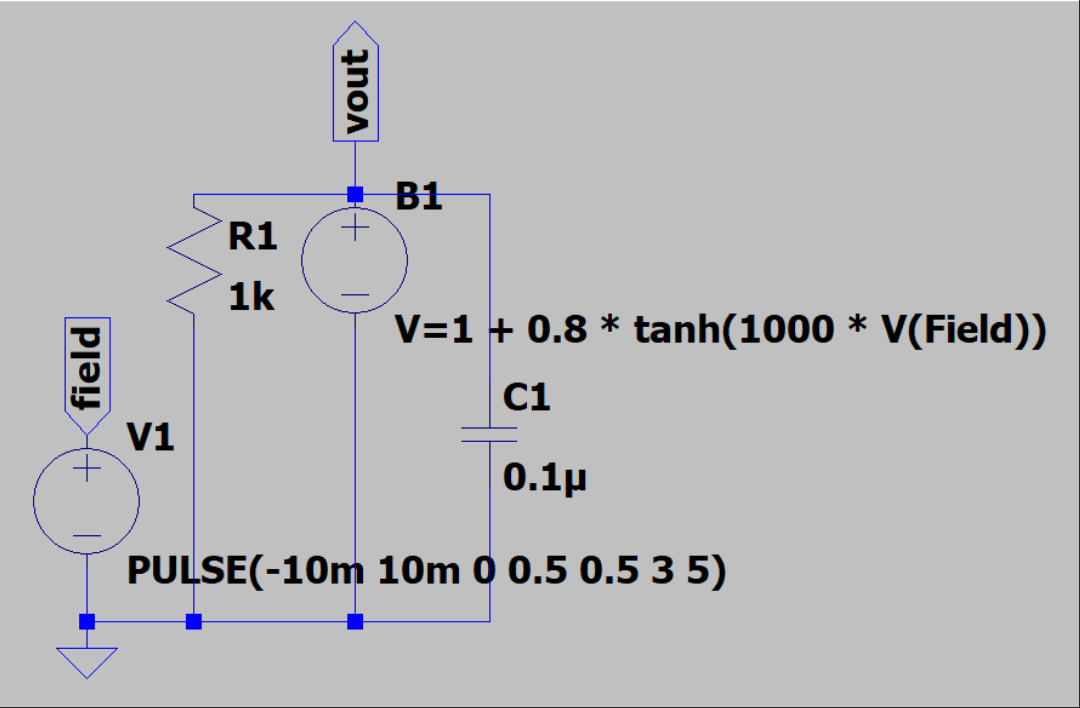
\includegraphics[width=0.6\textwidth]{subpages/images/magnet_model.png}
    \caption{LTspice Ideal Model of DRV5053}
    \label{fig:ideal_model}
\end{figure}
\begin{figure}[H]
    \centering
    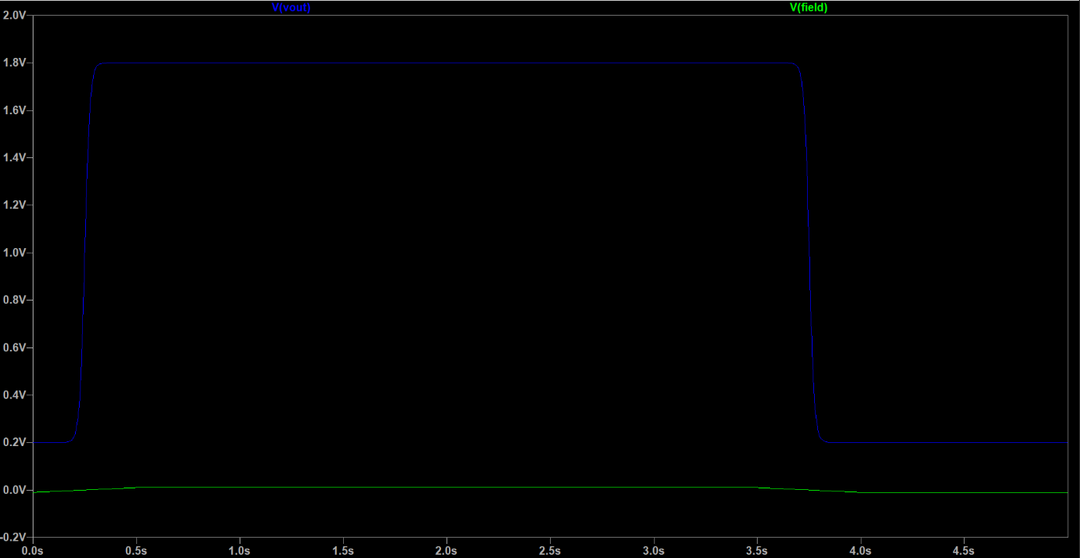
\includegraphics[width=0.6\textwidth]{subpages/images/magnet_out.png}
    \caption{Output of DRV5053 LTspice Model}
    \label{fig:model_output}
\end{figure}
These findings made it clear that additional signal conditioning would be necessary for reliable operation. The output required amplification to boost the detectable range.


\section{Amplification}
\begin{figure}[H]
    \centering
    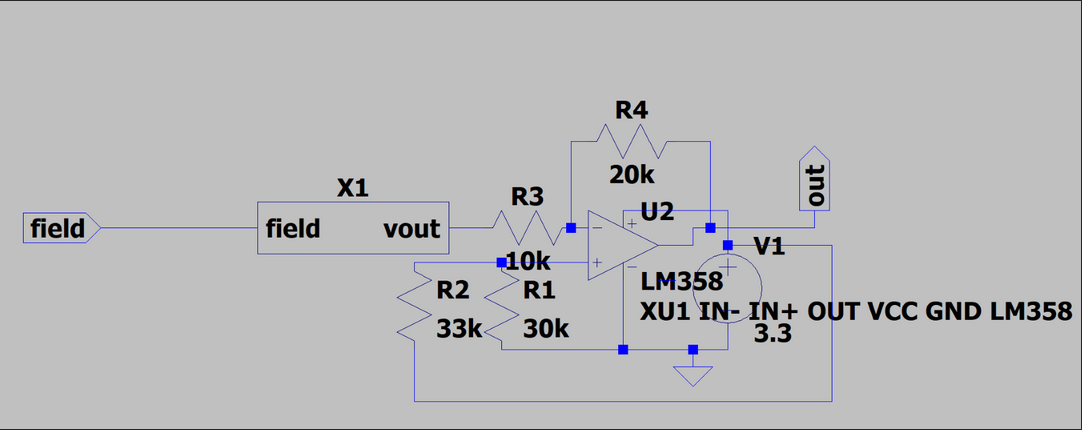
\includegraphics[width=0.6\textwidth]{subpages/images/magnet_circuit.png}
    \caption{Final Circuit Diagram}
    \label{fig:circuit}
\end{figure}
The amplification stage plays a critical role in ensuring reliable detection of the duck's magnetic field. The LM358 operational amplifier, configured as an inverting amplifier with a gain of -10, is illustrated in Figure 7.3. It uses a 10kΩ input resistor and 100kΩ feedback resistor to boost the Hall sensor's weak 0.2V-1.8V output to a more usable 0V-3.3V range compatible with the Metro M0's ADC inputs. The circuit includes a 1.1V virtual ground reference to enable proper single-supply operation by effectively creating a mid-supply point for the op-amp's inputs and outputs. Careful design ensures the amplified signal remains within the 0V-3.3V range, significantly improving the system's ability to detect and classify ducks at distances up to 6.5cm - a huge improvement over the raw Hall sensor output.
\begin{table}[H]
    \centering
    \begin{tabular}{|c|c|c|}
        \hline
        \textbf{Offset (V)} & \textbf{Gain (mV)} & \textbf{Distance (cm)} \\
        \hline
        1.1                 & -4.7               & 3.5                    \\
        \hline
        1.1                 & -6.8               & 4.5                    \\
        \hline
        1.1                 & -10                & 6.5                    \\
        \hline
    \end{tabular}
    \caption{Hall Sensor Output vs Distance}
    \label{tab:hall_output_distance}
\end{table}

\section{Building and Testing}
The final assembled circuit for the Hall sensor and amplification stage is shown in Figure 7.4.

Comparing these experimental results with the ideal LTspice simulations (Figures 7.1 and 7.2), it's evident that while the simulations provided a theoretical understanding of the sensor's behaviour, real-world conditions presented additional challenges. They did not account for the rapid signal attenuation over distance that was observed in physical testing.
\begin{figure}[H]
    \centering
    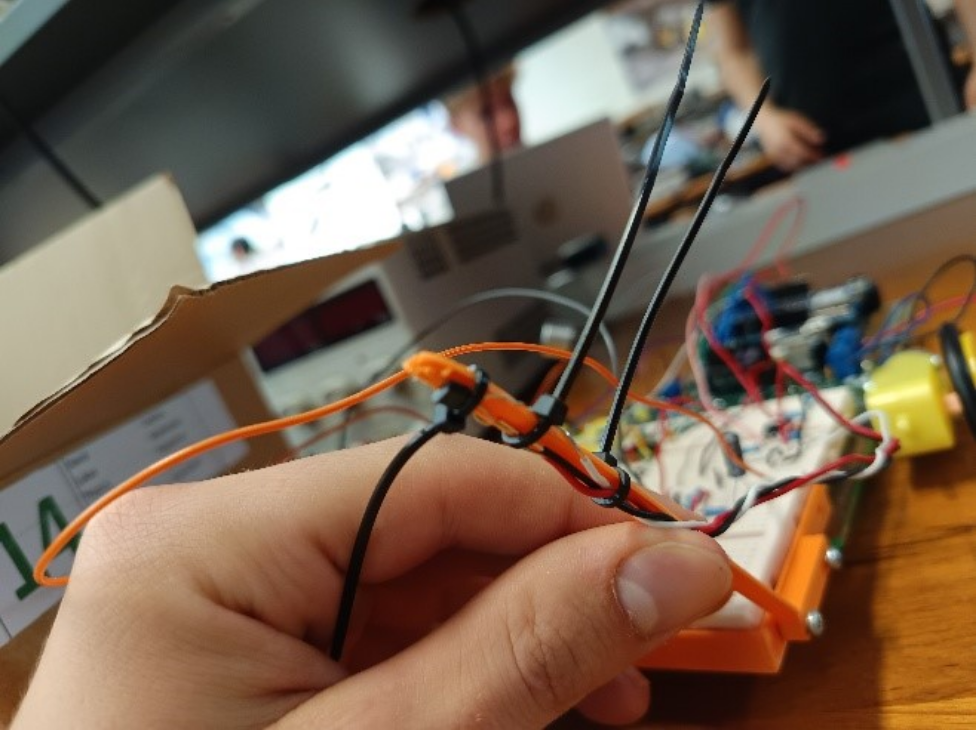
\includegraphics[width=0.7\textwidth]{subpages/images/magnet_arm_irl.png}
    \caption{Arm for Hall Sensor}
    \label{fig:magnet_arm}
\end{figure}
\begin{figure}[H]
    \centering
    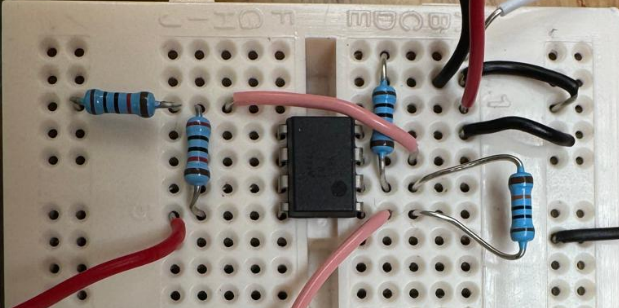
\includegraphics[width=0.7\textwidth]{subpages/images/magnet_circuit_irl.png}
    \caption{Final Circuit}
    \label{fig:circuit_irl}
\end{figure}
Since the magnet is placed facing up inside the duck’s head, the sensor needs to face the top of the duck’s head to detect the magnetic field. To implement this, we 3D printed an arm for the sensor to position it over the duck.

The need for amplification, as demonstrated by the improved detection distances in the table, was a direct consequence of these real-world limitations, highlighting the gap between ideal simulation and practical implementation. While the ideal model showed a clean signal, the physical setup necessitated amplification to achieve robust performance, especially at weaker magnetic fields. The discrepancy between simulated ideal conditions and physical testing underscores the importance of iterative design and validation, where simulations provide a baseline, and practical experiments reveal critical design requirements like amplification.

\chapter{Arduino and CAD Integration}
\section{Arduino Code}
To ensure the EESeaboat ("rover") operates reliably, the Arduino firmware has been designed to be lean and resilient. The Arduino does not render a webpage or handle interface concerns; its sole responsibility is processing movement and sensor requests via a simple HTTP server.

The system is designed with a clear separation between control logic and the user interface, where the Arduino acts as an HTTP server, listening for specific GET requests. The web interface (a JavaScript-based frontend) sends commands and displays responses.

This approach allows the user interface to operate independently of the rover hardware, resulting in a clear division of responsibilities:

\begin{figure}[h]
  \centering
  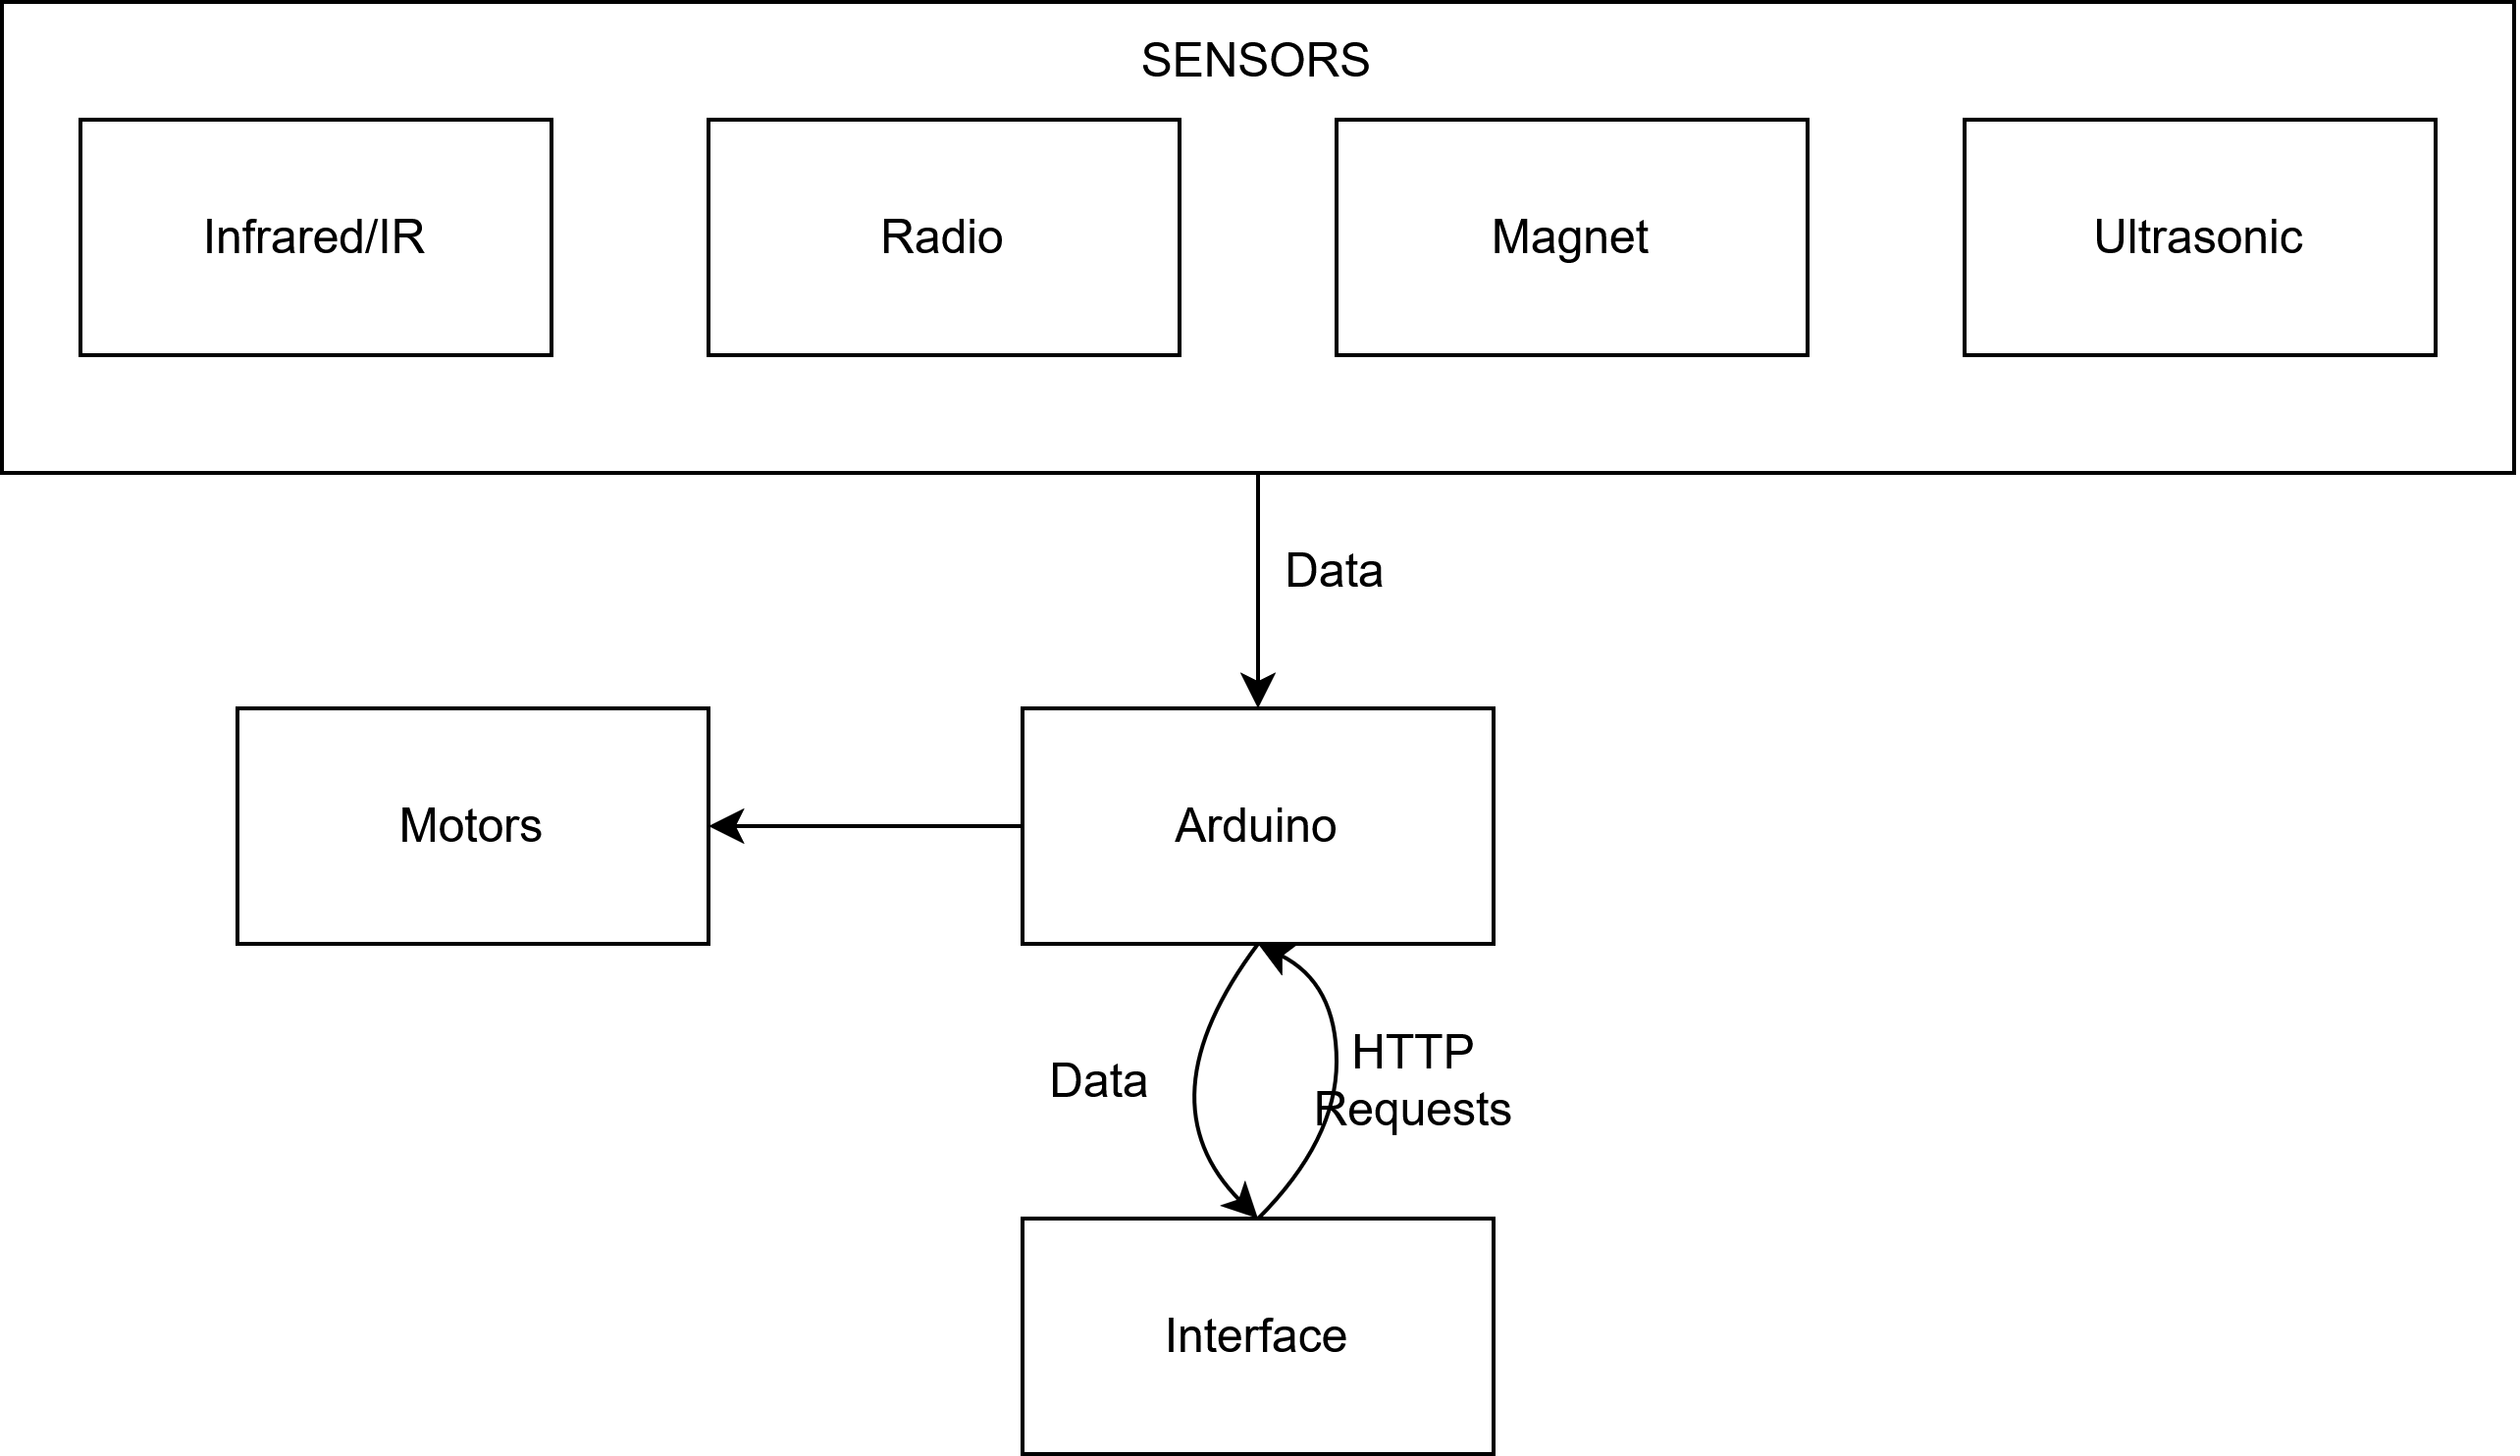
\includegraphics[width=0.8\textwidth]{subpages/images/arduino_data_flows.png}
  \caption{Data Flows Diagram}
  \label{fig:data_flows}
\end{figure}

\subsection*{Arduino as an HTTP Server}
The Arduino uses the \texttt{WiFiWebServer} library to create an HTTP server. Specific URL routes are mapped to functions using \texttt{server.on()}. Each route corresponds to a command or sensor request. A few movement examples are listed below:

\begin{verbatim}
server.on(F("/forward"), moveForward);
server.on(F("/back"), moveBack);
server.on(F("/left"), moveLeft);
server.on(F("/right"), moveRight);
server.on(F("/stop"), moveStop);
\end{verbatim}

Similar routes exist to request data from the sensors. Each function follows the same overall structure, inspired by subroutines which have a general header, body, and general exit:
\begin{itemize}
  \item Logs the received command to the Serial Monitor for debugging.
  \item Executes the main body of the specific function.
  \item Responds with an HTTP status and text message.
\end{itemize}

As an example, moving left is defined as below:

\begin{verbatim}
void moveLeft()
{
  Serial.println(F("[INFO] Command: Move Left"));
  digitalWrite(leftMotorPin, LOW);
  digitalWrite(rightMotorPin, HIGH);
  digitalWrite(leftMotorDirPin, HIGH);
  digitalWrite(rightMotorDirPin, HIGH);

  server.sendHeader("Access-Control-Allow-Origin", "*");
  server.send(200, F("text/plain"), F("Moving Left"));
}
\end{verbatim}

This pattern ensures each route is stateless and compatible with asynchronous HTTP communication.

Additional routes were defined to handle sensor readings. These include:
\begin{itemize}
  \item \texttt{/IR} - Returns the frequency of the infrared sensor.
  \item \texttt{/radio} - Returns the frequency of the radio signal.
  \item \texttt{/magnet} - Returns the magnetic direction (NORTH/SOUTH).
  \item \texttt{/ultra} - Returns a duck’s name embedded in the ultrasonic data.
\end{itemize}

Each handler processes the sensor reading and sends back a text response in a consistent, parseable format (e.g., \texttt{"457Hz"} or \texttt{"Name: Wibbo"}).

\subsection*{Web Interface}
\begin{figure}[h]
  \centering
  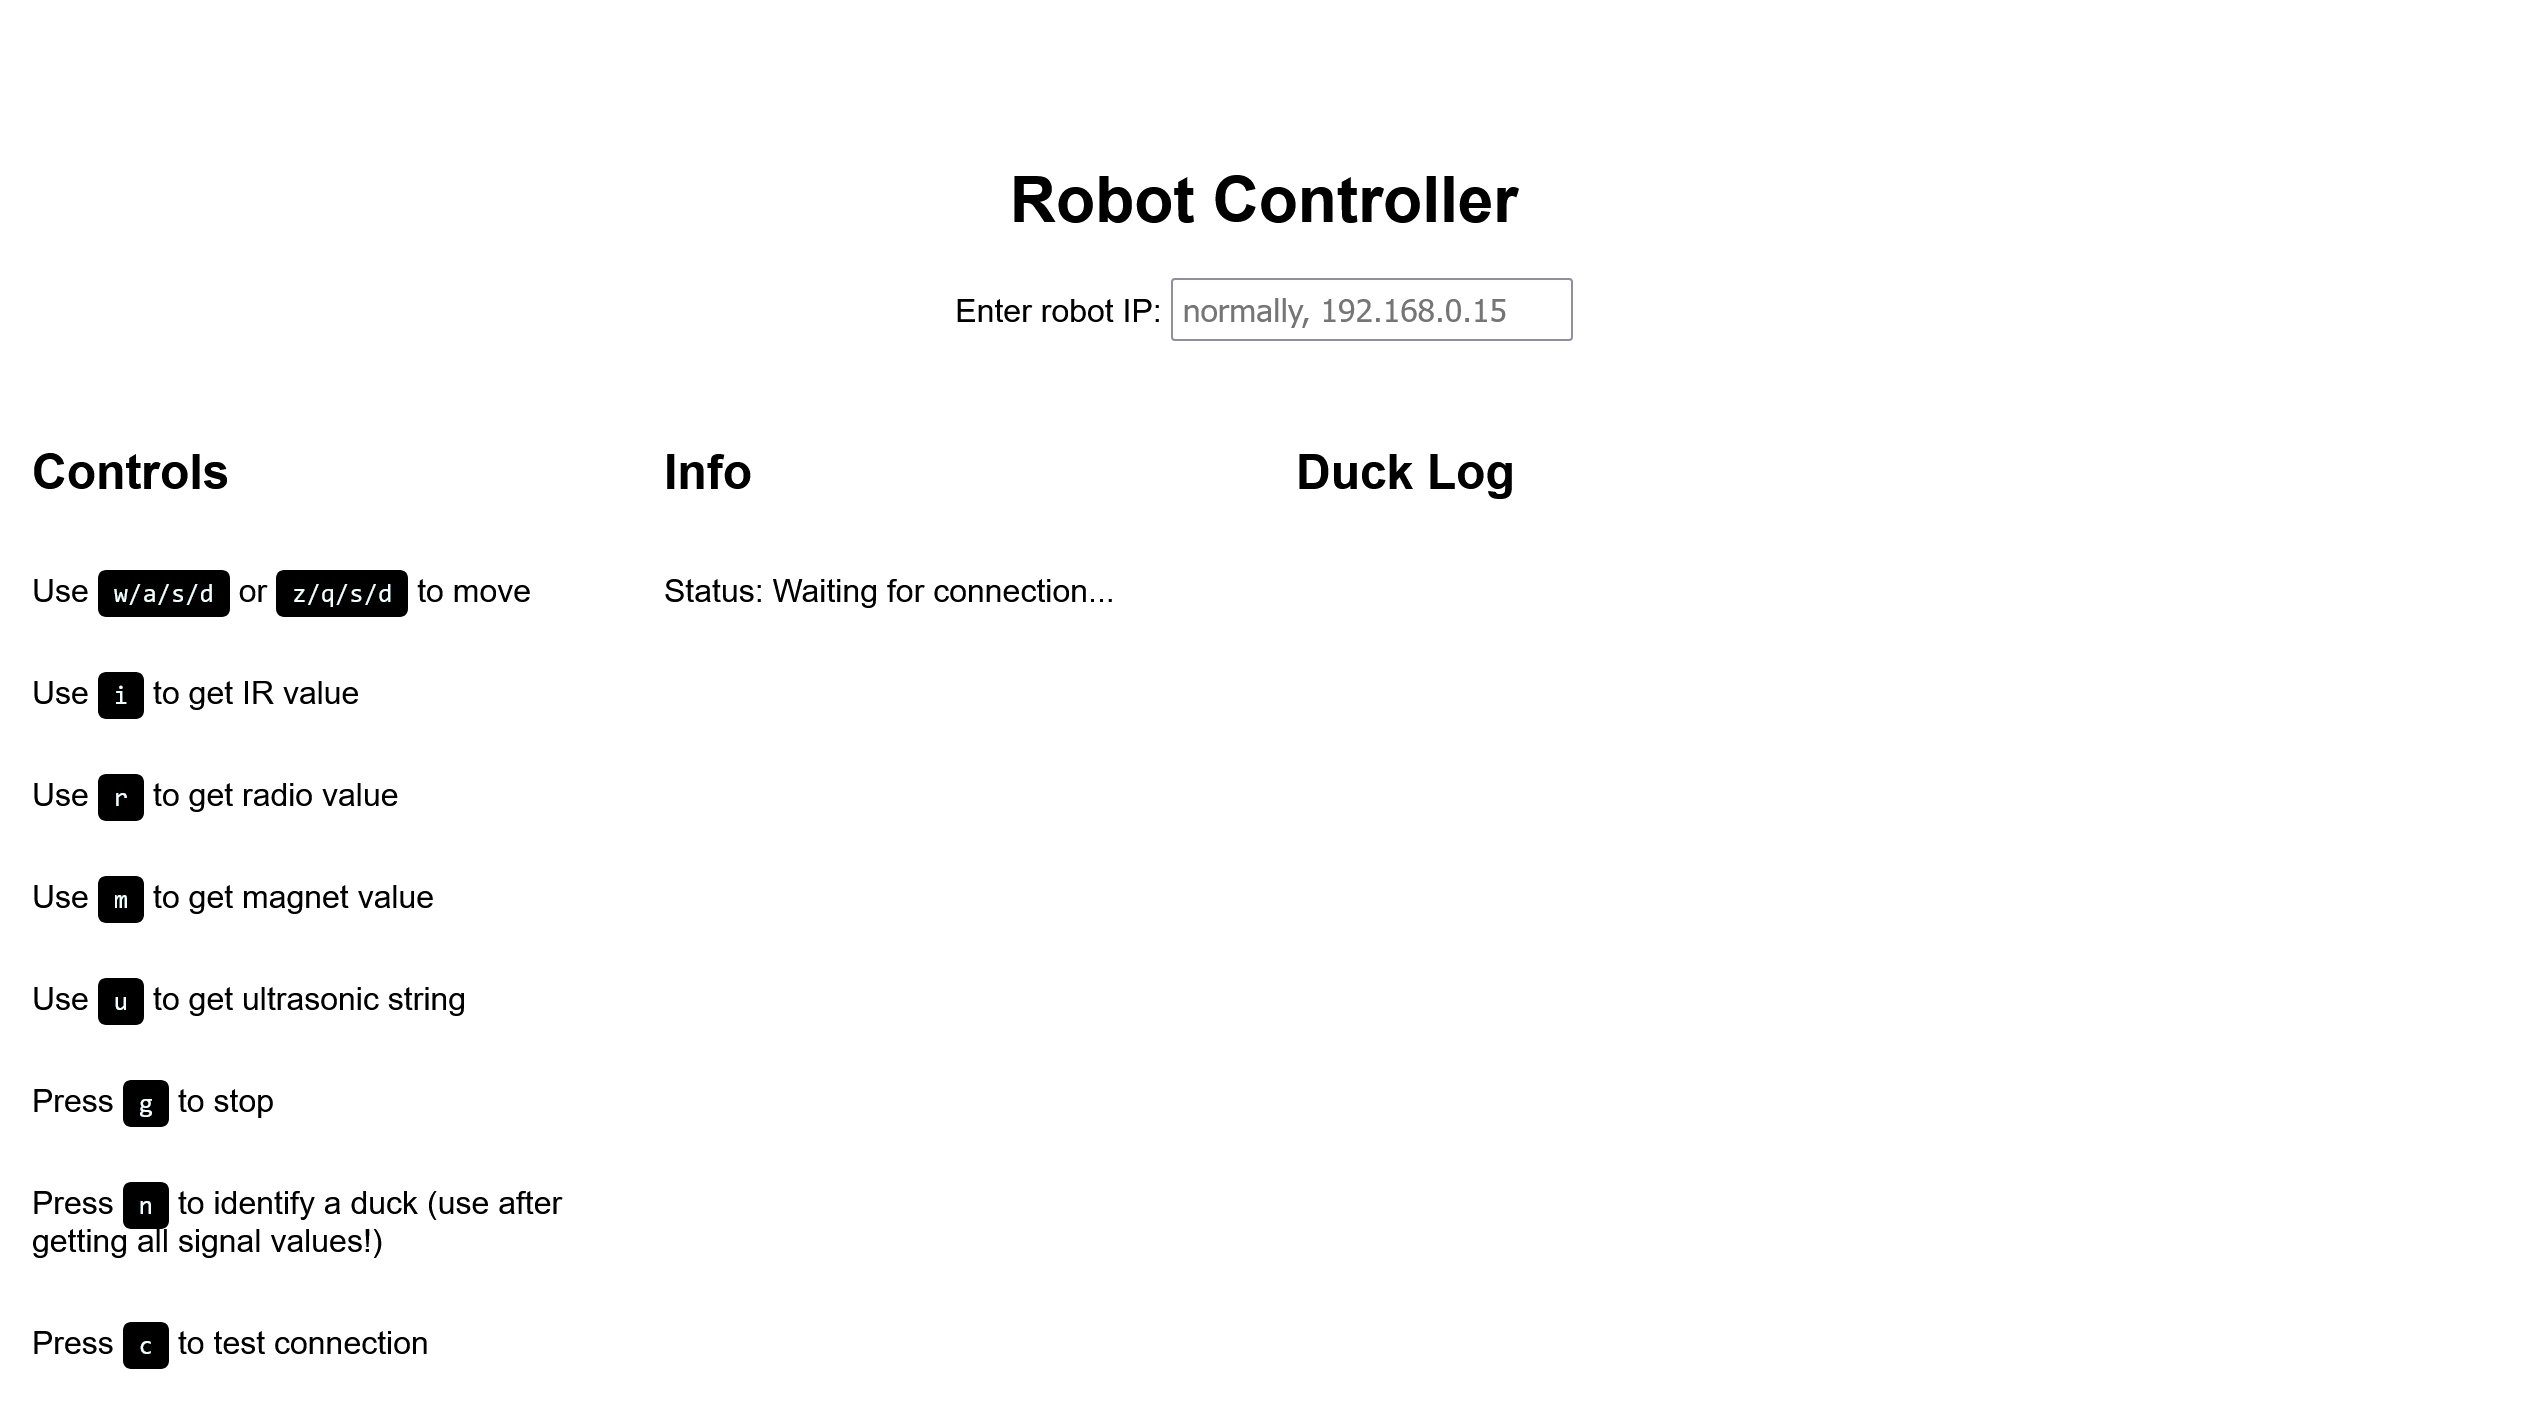
\includegraphics[width=0.8\textwidth]{subpages/images/early_web_interface.png}
  \caption{Early Version of User Interface}
  \label{fig:early_web_interface}
\end{figure}

The front-end is a JavaScript-based web application. It uses keyboard input to send commands to the rover over HTTP, using the \texttt{fetch()} API. The user specifies the rover’s IP address, then interacts using intuitive keybindings (\texttt{wasd} for movement and initials for other). The script tracks active keys and suppresses duplicate requests, especially for movement commands, to minimize redundant traffic.

\begin{verbatim}
fetch(`http://${ip}/${command}`)  
      .then(res => res.text())  
      .then(text => {  
          statusDisplay.textContent = text;  
   // ... more here ...  
      })  
      .catch(err => {  
          console.error(err);  
          statusDisplay.textContent = "Failed to connect";  
      });
\end{verbatim}

This function is responsible for funneling user interaction to send the correct request to the Arduino.

\subsection*{Duck Identification}
To classify ducks, each has a species-specific sensor signature comprising:
\begin{itemize}
  \item Infrared frequency
  \item Radio frequency
  \item Magnetic orientation
\end{itemize}

The identification logic maps these attributes to known species using tolerance-based matching. The logic table from the project brief is encoded as follows:

\begin{center}
  \begin{tabular}{|c|c|c|c|}
    \hline
    Species & Infrared & Radio & Magnetic \\
    \hline
    Wibbo   & 457Hz    &       & Down     \\
    Gribbit &          & 100Hz & Down     \\
    Snorkle & 293Hz    &       & Up       \\
    Zapple  &          & 150Hz & Up       \\
    \hline
  \end{tabular}
\end{center}

We keep these variables in the code:
\begin{verbatim}
let magnetDir = "";
let irFreq = 0;
let radioFreq = 0;
let duckName = "";
\end{verbatim}

Upon pressing the \texttt{n} key, the function \texttt{newDuck()} checks against the table:
\begin{verbatim}
const TOLERANCE = 10;
if (Math.abs(irFreq - 457) <= TOLERANCE && magnetDir === "SOUTH") {
  species = "Wibbo";
} else if (Math.abs(radioFreq - 100) <= TOLERANCE && magnetDir === "SOUTH") {
  species = "Gribbit";
} else if (Math.abs(irFreq - 293) <= TOLERANCE && magnetDir === "NORTH") {
  species = "Snorkle";
} else if (Math.abs(radioFreq - 150) <= TOLERANCE && magnetDir === "NORTH") {
  species = "Zapple";
}
\end{verbatim}

The species name and duck name are then timestamped and inserted into the “Duck Log” section of the UI. If no match is found, the user is prompted to verify that all sensor readings have been collected.

\subsection*{Sensor Processing}
Each sensor on the rover provides a signal for duck classification and is accessed via a dedicated HTTP route. The Arduino reads the sensor data, processes it as needed, and returns a plain-text response that the browser can easily interpret. Not shown here is code for error handling, which is done by sending an HTTP status 400 and an error string to the interface if there is no output from sensors, or if the output doesn’t match expected outcomes.

\subsubsection*{Infrared and Radio Frequency Sensors}
Both the infrared and radio sensors are connected to analog input pins. The Arduino measures their signal frequency using the \texttt{pulseIn()} function and computes the corresponding Hertz value, by measuring the high and low time to get the period. A simplified version of the functionality is shown below:

\begin{verbatim}
float getFreq(int pin) {
  unsigned long highTime = pulseIn(pin, HIGH, 50000);
  unsigned long lowTime = pulseIn(pin, LOW, 50000);
  if (highTime == 0 || lowTime == 0) return 0;
  return 1000000.0 / float(highTime + lowTime);
}
\end{verbatim}

This then gets sent to the interface through each respective route, a frequency string like \texttt{"457.00Hz"} that the JavaScript interface extracts and compares to known species ranges.

\subsubsection*{Magnetic Sensor}
The rover uses a Hall effect sensor to detect the magnetic's field polarity. The Arduino reads an analog voltage that varies depending on the pole facing the sensor.

\begin{verbatim}
int rawValue = analogRead(magnetPin);
float voltage = rawValue * (3.3 / 1023.0);
\end{verbatim}

The sensor outputs roughly 2.5V with no field, >2.05V for South polarity (DOWN), and <1.98V for North polarity (UP). Based on this, the Arduino classifies the magnetic direction:

\begin{verbatim}
if (voltage >= 2.05) {
  server.send(200, "text/plain", "SOUTH");
} else if (voltage <= 1.98) {
  server.send(200, "text/plain", "NORTH");
} else {
  server.send(400, "text/plain", "ERROR: Invalid magnet reading");
}
\end{verbatim}

This method is more precise than using a binary input and allows detection even with weak magnetic fields. The output is returned as \texttt{"NORTH"} or \texttt{"SOUTH"} for frontend classification logic.

\subsubsection*{Ultrasonic Sensor}
The ultrasonic system transmits a 4-character string over a slow UART serial link (e.g., \#Eve). The Arduino waits for the start character, ‘\#’ and then reads the remaining three letters as the name. It uses \texttt{Serial1} to read the signal at a baud rate of 600 to match the bit rate of the signal.

The process is robust against garbage data and timeouts:

\begin{verbatim}
while (!foundStart && (millis() - startTime < 1000)) {
  if (Serial1.available()) {
    charIn = Serial1.read();
    if (charIn == '#') {
      name += charIn;
      foundStart = true;
    }
  }
}
\end{verbatim}

After receiving the start marker, the remaining characters are read one at a time with small delays to accommodate the slow baud rate:

\begin{verbatim}
while (name.length() < 4) {
  if (Serial1.available()) {
    charIn = Serial1.read();
    name += charIn;
  }
}
\end{verbatim}

The name then gets returned to the interface to continue the duck identification.

\subsection*{Movement}
Using the given H-Bridge Motor Driver Module, we can connect the corresponding pins for each motor’s movement and direction to inputs to the Arduino. Then, depending on the movement command received, the motors are driven at appropriate speeds and directions using the following function:

\begin{verbatim}
void setMotorSpeed(int leftSpeed, int rightSpeed, bool leftForward, 
bool rightForward)
{
  analogWrite(leftMotorPin, leftSpeed);
  analogWrite(rightMotorPin, rightSpeed);
  digitalWrite(leftMotorDirPin, leftForward ? HIGH : LOW);
  digitalWrite(rightMotorDirPin, rightForward ? HIGH : LOW);
}
\end{verbatim}

Using \texttt{analogWrite} for the speed, we can drive motors at different voltages to allow for diagonal movement.

\section{CAD}
To keep things simple with the design, we used the given chassis, which allowed us to spend more time working on the more pressing issues. However, we knew that space would be tight if we didn’t add anything to the original chassis. We wanted to push the chassis to the extreme, so we looked at what was available to be worked with. The chassis has two holes at the front, originally meant for servo motors. We decided to repurpose these to place a mount, which would hold our ill-fitting circuitry and all the sensors. A thing to keep in mind here was the weight, as the original chassis is already close to half the permitted weight, something kept in mind throughout the project.

In total four parts where designed and added to the chassis to allow for proper operation of the rover.

\subsection*{Breadboard Box and Infrared Sensor Shield}
\begin{figure}[H]
  \centering
  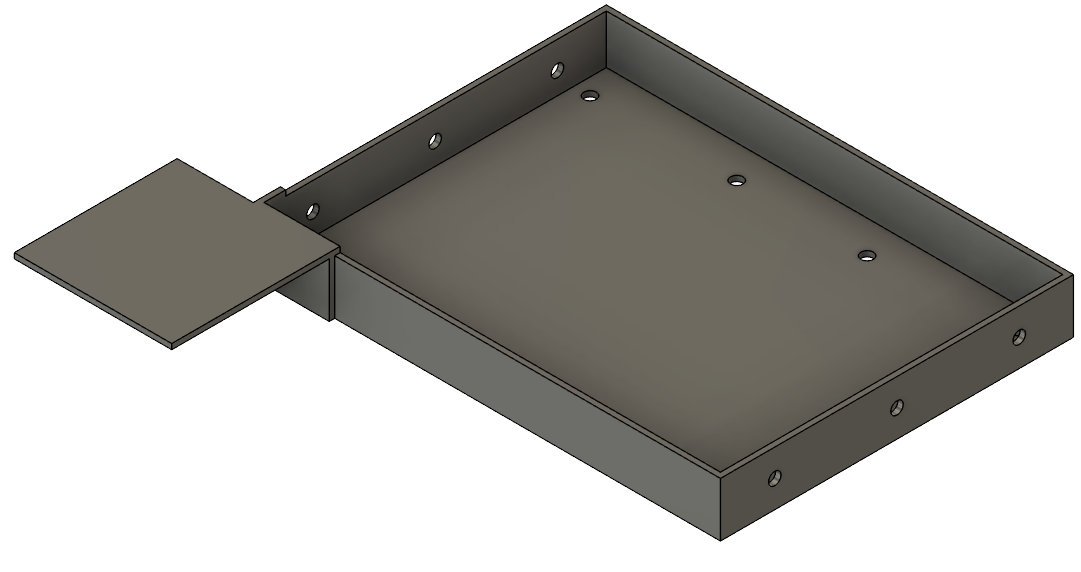
\includegraphics[width=0.7\textwidth]{subpages/images/breadboard_box.png}
  \caption{Mount for Breadboard with a Shield for Phototransistor}
  \label{fig:breadboard_box_shield}
\end{figure}
This enclosure accommodates a breadboard for additional circuit components, enabling larger and cleaner circuit layouts by providing extra space for separation and organization. The box includes a dedicated side mounting points for the infrared and other sensor, and features a cover designed to shield the infrared sensor from ambient light interference, thereby improving measurement accuracy.

\subsection*{Magnetic Sensor Arm Mount}
\begin{figure}[H]
  \centering
  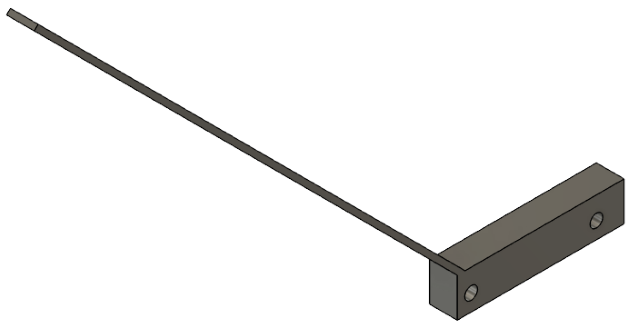
\includegraphics[width=0.7\textwidth]{subpages/images/magnet_arm.png}
  \caption{Arm Mount for the Hall Sensor}
  \label{fig:magnet_arm}
\end{figure}
To optimize detection, the magnetic sensor must be positioned above the duck’s head. A vertical arm was designed to elevate the sensor to the correct height while anchoring it to the box, ensuring consistent alignment during operation.

\subsection*{Ultrasonic Sensor Housing}
\begin{figure}[H]
  \centering
  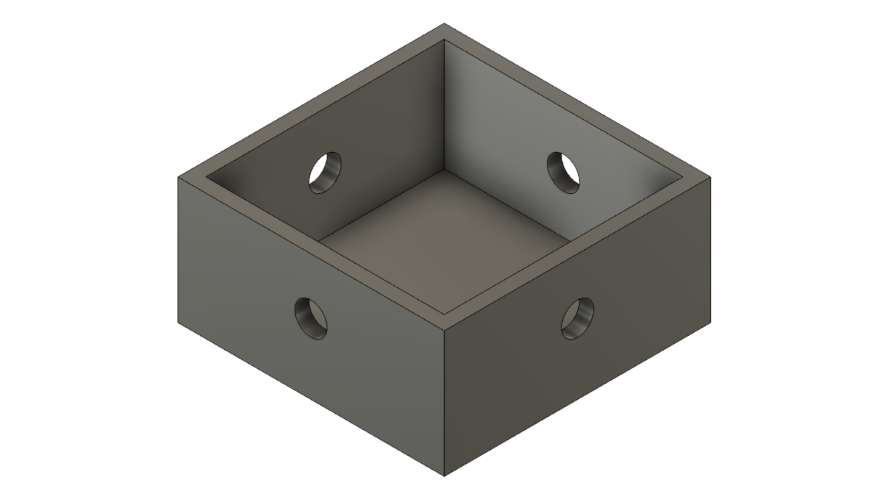
\includegraphics[width=0.7\textwidth]{subpages/images/ultrasonic_mount.png}
  \caption{Holder for the Ultrasonic Sensor}
  \label{fig:ultrasonic_mount}
\end{figure}
Due to form factor limitations, the ultrasonic sensor could not be mounted directly to the chassis. A dedicated enclosure was designed with pass-through holes for wiring, providing a secure mounting location and easy access to the sensor for UART signal processing.

\chapter{Conclusion}
On balance, there is a clear establishment of the fact that a practical project will always have a multitude of avenues to go about handling it. Though analogue methods seem less alien given the theory covered this year, thorough research and discussion led the group to believe that digital methods supersede in terms of efficiency and scalability.

With society accelerating towards a singularity of a ubiquitous realm, electrical, electronic and information engineering continue to have undeniable impacts on our world. As demonstrated in this project, detection systems require thorough design and acknowledgement of requirements and restrictions, which is a skill needed even in real-world projects involving search and rescue mechanisms or studying species in unchartered terrain. To add contextual relevance onto this project, we can consider swarm robotics - a recently emerging field of technological research aiming to produce a network of robots which mimic the herd mentality of natural swarms such as insects. By having multiple robots coordinating and working simultaneously to complete tasks, efficiency soars without the need for one entity to control everything. In a similar sense, our project, beyond the task expectations, could have involved multiple rovers detecting different waves, but all communicating in parallel to receive and analyse data faster.

From a focussed perspective, this project utilized a range of hardware and software components. The hardware included operational amplifiers, diodes, oscilloscopes, microcontroller and a range of resistors and capacitors. Meanwhile, the software incorporated full-stack development using the Arduino as the server, and the interface as the front-end, while team skills in LTspice and 3D printing with Fusion360 were simultaneously developed.

Reflecting, despite the absences and reduced team size, members communicated well, helped explain complex concepts such as UART protocol to each other and ensured all strengths were exploited. Regardless of task allocation, the team ensured all members had a fair understanding of all sections such that everyone had a holistic view of this group project. With knowledge of digital electronics, computer architecture and circuit design, this first year rover project was successful, abided by the guidelines and provided an opportunity to place theory into a practical domain under time constraints.

\chapter{Project Evaluation and Future Actions}
\begin{enumerate}
    \item Ultrasound -- Optimising the gain in the circuit when receiving the ultrasonic signal, allowing for detection at a further range.
    \item Arduino -- Should send separate messages to interface with display text and information for duck detection, instead of extracting information from the original text response.
    \item CAD -- Designs had to be redone due to strain from weight (such as magnetic arm), something that should've been considered beforehand.
    \item Radio -- Could have trialled the coil antenna and collected results to compare it against the inductor to see how different the two methods were.
    \item Infrared -- With better time management, a thorough investigation would have built the bandpass filters as well and tested for efficiency by comparing the analogue and digital methods. The phototransistor taken was from the EEBug, but perhaps the remaining 17\% of the budget could have been contributed towards purchasing a more powerful or sensitive phototransistor to ensure clearer signals and smoother detection.
    \item Magnetic --     Could have benefited from a dynamic gain amplification stage. Instead of a fixed gain, an adaptive gain control system would allow the amplifier to automatically adjust its amplification based on the detected magnetic field strength. This would optimize sensitivity for weak, distant signals while preventing saturation from strong, close-range signals, maximizing the effective detection range.
    \item Budgeting -- The cumulative budget came out to £50, but this could have been avoided through better op-amp research (see Table~\ref{tab:component_orders}).
\end{enumerate}

\begin{table}[H]
    \centering
    \small
    \makebox[\textwidth]{%
        \begin{tabular}{|p{5cm}|l|r|r|r|}
            \hline
            \textbf{Description}                   & \textbf{Unit Price (£)} & \textbf{Quantity} & \textbf{Line Sum (£)} \\
            \hline
            MCUSD16A40S12RO Ultrasonic transceiver & 1.76                    & 1                 & 1.76                  \\
            1N4148 Diode                           & 0.04                    & 5                 & 0.20                  \\
            MCP6021-I/P Opamp                      & 1.34                    & 2                 & 2.68                  \\
            DRV5053OAQLPG Hall Effect Sensor       & 0.65                    & 1                 & 0.65                  \\
            LM358N/NOPB Opamp                      & 0.66                    & 1                 & 0.66                  \\
            LM6142BIN/NOPB Opamp                   & 6.94                    & 3                 & 20.82                 \\
            OPA703PA Opamp                         & 4.73                    & 5                 & 23.65                 \\
            LM324N Opamp                           & 0.28                    & 1                 & 0.28                  \\
            \hline
        \end{tabular}
    }
    \caption{Component Orders and Costs}
    \label{tab:component_orders}
\end{table}




\end{document}
